\documentclass[12pt,a4paper,openright]{article}

%\\usepackage\{url,graphicx\}\
\usepackage[pdftex]{graphicx}
\usepackage[bookmarks,%
            a4paper,%
            breaklinks,%
            backref=true,%
            urlcolor=blue,
            linkcolor=blue,
            citecolor=magenta,
            pdfhighlight=/I,%
            pdffitwindow=true,%
            pdfstartview=Fit,%
            pdfcenterwindow=true,%
            pdfborder={0 0 0.5 [2 2]},
            linkbordercolor={0 0 0},%
            %colorlinks,%
            colorlinks=true,
            hyperfootnotes=false,
            %linkcolor={0 0 0},
            urlbordercolor={0 0 0},
            %pdfbordercolor=magenta,
            pdftitle=ADC Project Report,%
            pdfauthor=Francisco]%
            {hyperref}

\renewcommand\thefootnote{\textcolor{red}{\arabic{footnote}}}
\usepackage[english]{babel}
\usepackage[utf8]{inputenc}
\usepackage{amsmath}
\usepackage[margin=2cm]{geometry}
%\usepackage{fullpage}
\usepackage{setspace}
\usepackage{cleveref}
\usepackage{bm}
\onehalfspacing
\usepackage[font=small,labelfont=bf]{caption}
\usepackage{float}
\usepackage{booktabs}
\graphicspath{{expt/}}
%\usepackage[options]{natbib}
\usepackage{xfrac}
\usepackage{hyperref}
\usepackage{color}
\usepackage{epstopdf}
\usepackage{graphicx}
\usepackage{times}
\usepackage{indentfirst}
\usepackage[varg]{txfonts}
\usepackage{caption}
\usepackage{subcaption}
\renewcommand{\descriptionlabel}[1]{\hspace{\labelsep}\boldmath{\underline{#1:}}}
%
%\usepackage{listings}
%\usepackage{color} %red, green, blue, yellow, cyan, magenta, black, white
%\definecolor{mygreen}{RGB}{28,172,0} % color values Red, Green, Blue
%\definecolor{mylilas}{RGB}{170,55,241}
\usepackage[utf8]{inputenc} 

%\usepackage{subfig}
%\usepackage{footnotebackref}
\usepackage{footmisc}
%%% Macro definitions for Commonly used symbols
\newcommand{\etas}{\ensuremath{\eta_{\mathrm{s}}}}
\newcommand{\HRule}{\rule{\linewidth}{0.5mm}}




\begin{document}

\begin{titlepage}
\begin{center}
\textsc{\LARGE Royal Institute of Technology}\\[0.3cm]

\includegraphics[width=0.4\textwidth]{./logo}~\\[0.3cm]


\textsc{\Large PWC \\ Project Report}\\[0.5cm]

\HRule \\[0.4cm]
{ \huge \bfseries Project Report \\[0.4cm] }

\HRule \\[1.5cm]

\begin{minipage}{0.4\textwidth}
\begin{flushleft} \large
\emph{Authors:}\\
Alan \textsc{Anter} \\
Daniel \textsc{Bredstedt}\\
Sergio \textsc{Chávez Cárdenas}\\
Henrik \textsc{Forsell}\\
Johan \textsc{Ottersten}\\
Francisco \textsc{Rosário}\\
Jue \textsc{Zhang}\\

\end{flushleft}
\end{minipage}
\vfill
{\large \today}



\end{center}
\end{titlepage}

%\tableofcontents

% % % % % % % % % % % % % % % % % % % % % % % % % % % %
% % % % % % % % % % % % % % % % % % % % % % % % % % % %

%Beging of report 


\section{Theory}

Before implementation, it is important to study the possible coding and modulation schemes in order to predict the best combination for the given problem. In this section, the fundamentals of each technique are analysed.

\subsection{Modulation schemes}

\subsubsection{ASK}
Amplitude shift keying (ASK)uses the variations in amplitude of a carrier wave to represent the digital data. The mapping or assignment of $k$ information bits to the $M=2^k$ possible signal amplitudes may be done in different ways. The preferred assignment is the one in which the adjacent  signal amplitudes differ by one binary digit (Gray coding). The simplest case for the transmitted signal, when only two amplitudes exist, can be seen in figure(\ref{fig:ask}). 

\begin{figure}[h]
  \centering
    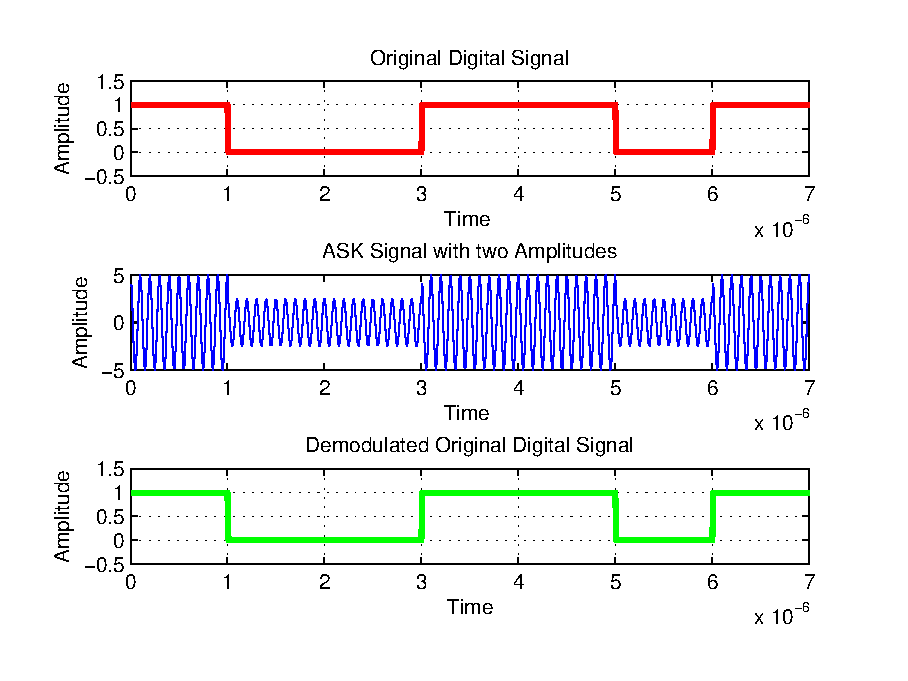
\includegraphics[width=0.7\textwidth]{ASKexample.eps}
    \caption{ASK modulation example in the absence of noise for amplitudes $a_1=2.5$ and $a_2=5$.}
    \label{fig:ask}
\end{figure}

It is important to have an high signal-noise to ratio (SNR), especially when the amplitudes are too close so that the demodulator can identify them. The ASK scheme is very sensitive to atmospheric noise, distortions and propagation conditions.  A possible demodulator is shown in figure (\ref{fig:askdem}).

\begin{figure}[h]
  \centering
    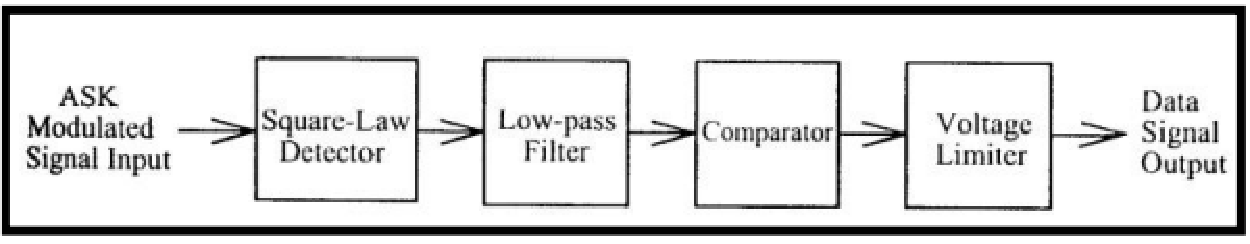
\includegraphics[width=0.7\textwidth]{askdem.pdf}
    \caption{Possible demodulator for ASK\protect\cite{ASKDemGaza}.}
    \label{fig:askdem}
\end{figure}

\subsubsection{FSK}
\label{subsec:fsk}
Frequency shift keying (FSK) is a modulation technique where the data is transmitted through discrete frequency changes of a carrier wave with fixed amplitude $A$. The simplest form is binary FSK (BFSK), where a sine wave $s_i(t)$ is transmitted per bit (as shown in figure(\ref{fig:fskex}). A $0$ or $1$ is transmitted as a sinusoid of frequency $f_0$ or $f_1$, respectively. 

\begin{figure}[h]
  \centering
    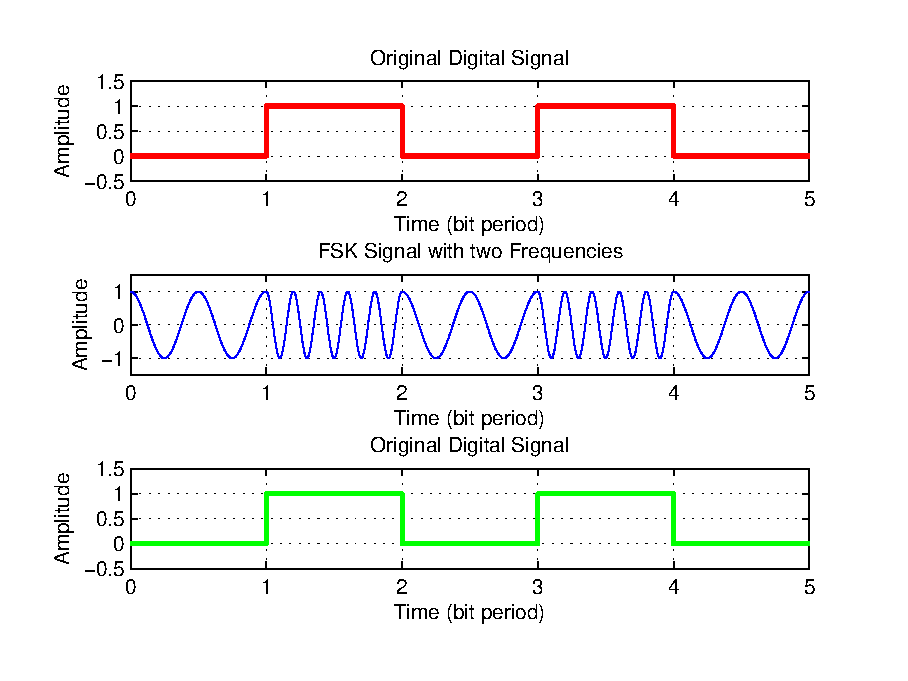
\includegraphics[width=0.7\textwidth]{fskexample.eps}
    \caption{BFSK example for 2 sinusoids of low frequency.}
    \label{fig:fskex}
\end{figure}

We can use multiple sinusoids of different frequencies to transmit $n$ bits, as well. In order to guarantee they are orthogonal, there should be $M=2^n$ frequencies separated by $\Delta f=\frac{k}{2T}$, where $k$ is an integer and $T$ is the bit period. Thereby, the complex baseband signalling waveforms for M-ary FSK are given by \cite{Madhow}:

\[{s_i}(t) = {e^{j2\pi {f_i}t}}{I_{[0,T]}},i = 1,2,...,M\]



In terms of demodulation, coherent and non-coherent methods exist and they depend on if the phase of the sinusoids $\phi$ are equal or not. Coherent demodulators consist of correlators (or matched filters, equivalently) and samples, but they require  synchronisation of the reference signals. The demodulator for the BFSK can be implemented with two correlators as shown in figure (\ref{fig:FSKdemcoherent}). This receiver is optimum in the sense that it minimizes the error probability for equally-likely binary signals. If a sinusoid with frequency $f_1$ is transmitted, for example, the upper correlator yields a signal $l_1$ with a positive signal component while $l_2$ has only a noise component, due to signals’ orthogonality.
  In case there is no chance of having a phase reference, then additional squarers or envelope detectors must be used for the non-coherent detection. In the last case, a minimum tone spacing of $\frac{k}{T}$ is required instead. The correlator implementation for non-coherent BFSK can be seen in figure (\ref{fig:FSKdemNoncoherent}).

 \begin{figure}[h]
 \centering
\begin{subfigure}[h]{0.9\textwidth}
 \centering
    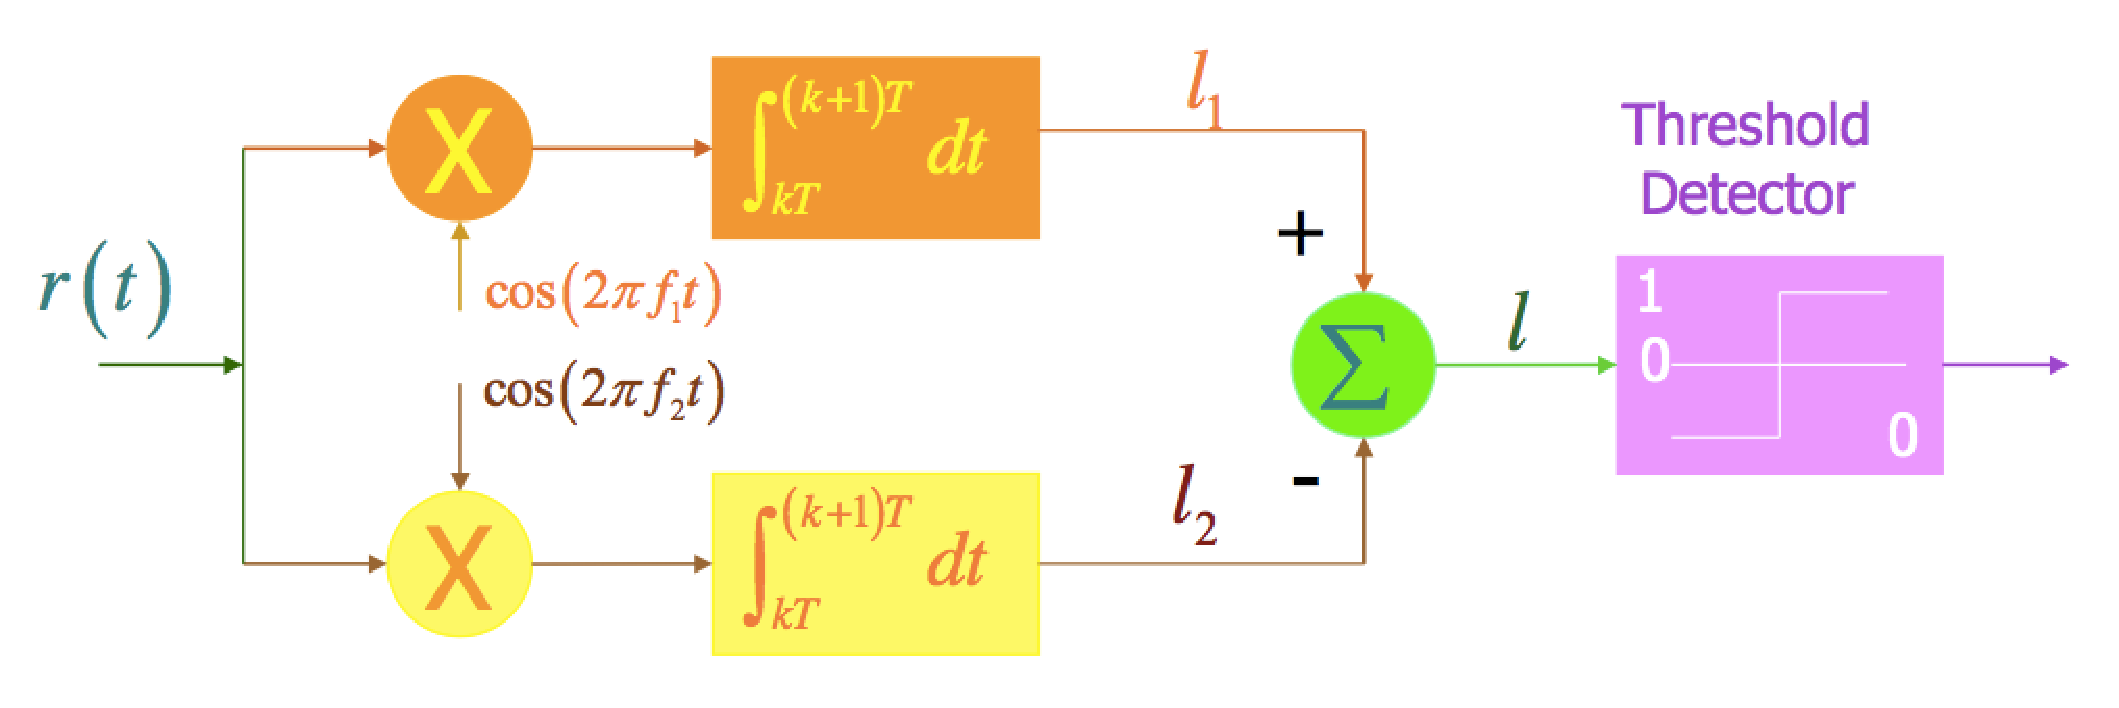
\includegraphics[width=0.6\textwidth]{fskdem1.pdf}
    \subcaption{Coherent.}
    \label{fig:FSKdemcoherent}

\end{subfigure}
\quad

\begin{subfigure}[h]{0.9\textwidth}
 \centering
    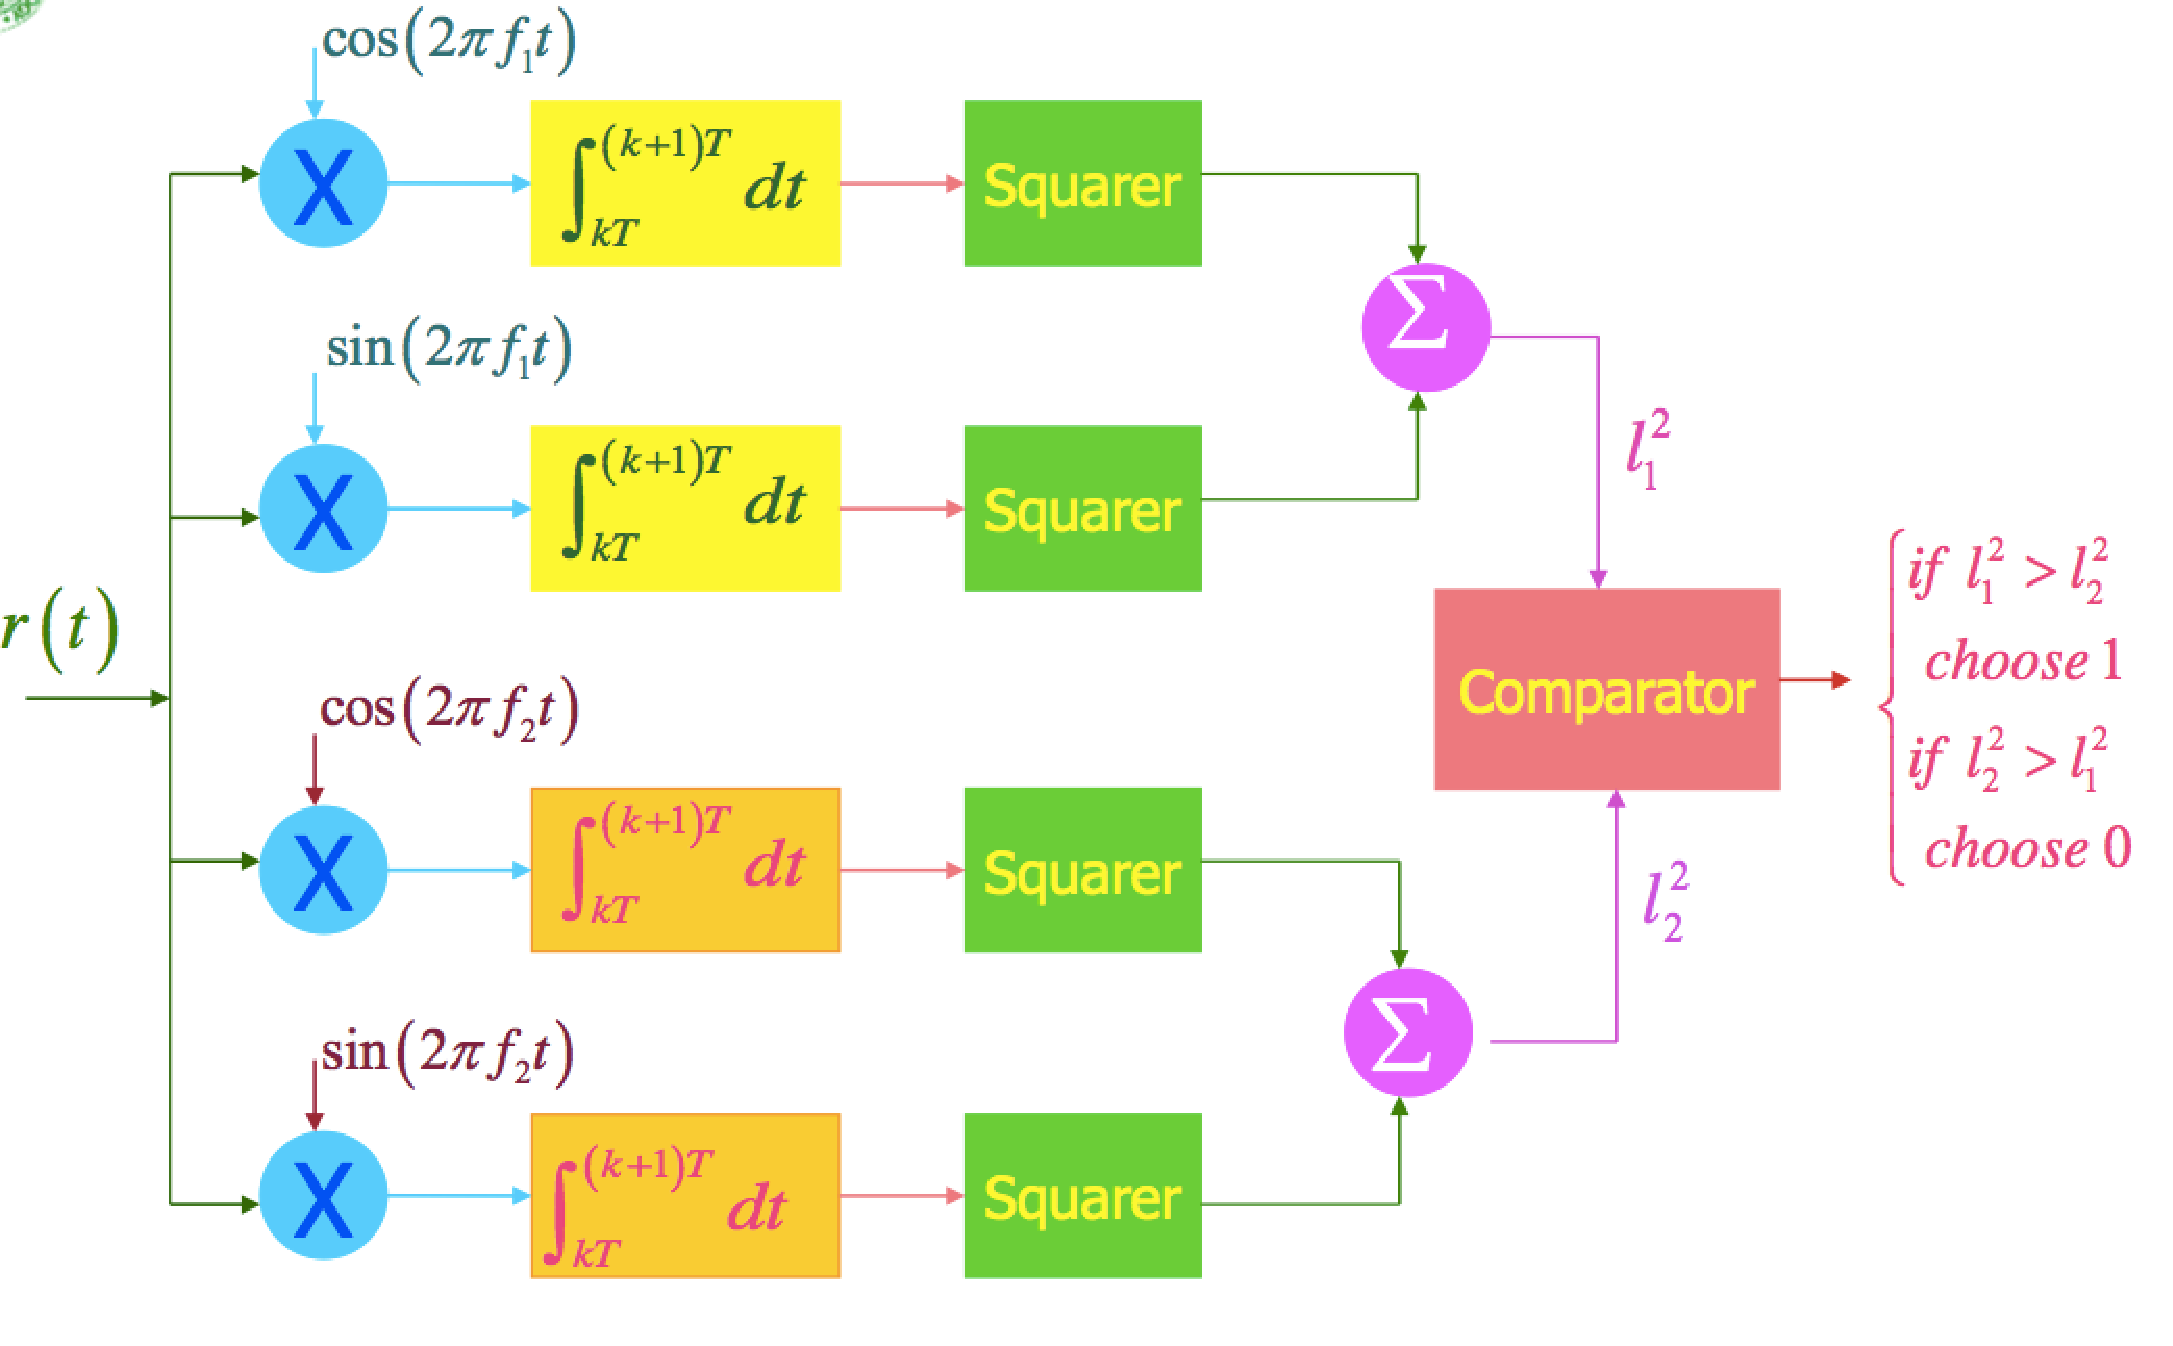
\includegraphics[width=0.6\textwidth]{fskdem2.pdf}
    \subcaption{Non-coherent.}
    \label{fig:FSKdemNoncoherent}
    \end{subfigure}
    \caption{Possible Demodulators for FSK \protect\cite{DigModTech}.}
\end{figure}


It is expected that the error performance for the non-coherent receivers is inferior to that of the coherent ones. However, the degradation in only a fraction of a dB. Other options for demodulation are available, such as the use of FFT schemes for peak picking or bandpass filtering at the used frequencies. 
The main advantages of this modulating scheme are: the in-sensitiveness to amplitude variations in the channel, its compatibility with non-linear transmitter and receiver systems, and that it is not a requirement to have an absolute frequency accuracy for correct demodulation (making it tolerant to local oscillators, drifts and Doppler shifts). One of the drawbacks is the fact that such scheme is less bandwidth efficient when compared with others like ASK or PSK. To avoid undesirable spectral characteristics(which could cause adjacent channel interference), continuous phase FSK is required (see figure \ref{fig:comparecpfsk} for comparison).

 \begin{figure}[h]
 \centering
	\begin{subfigure}[h]{0.9\textwidth}
 \centering
    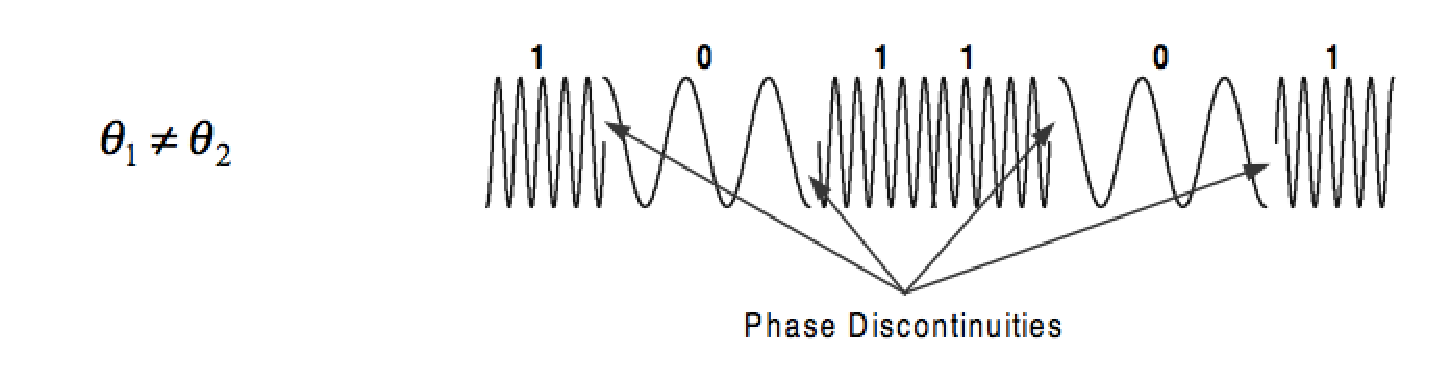
\includegraphics[width=0.6\textwidth]{ncpfsk.pdf}
    \subcaption{Non continuous phase FSK.}
    \label{fig:FSKcoherent}

	\end{subfigure}
	\quad

	\begin{subfigure}[h]{0.9\textwidth}
 	\centering
    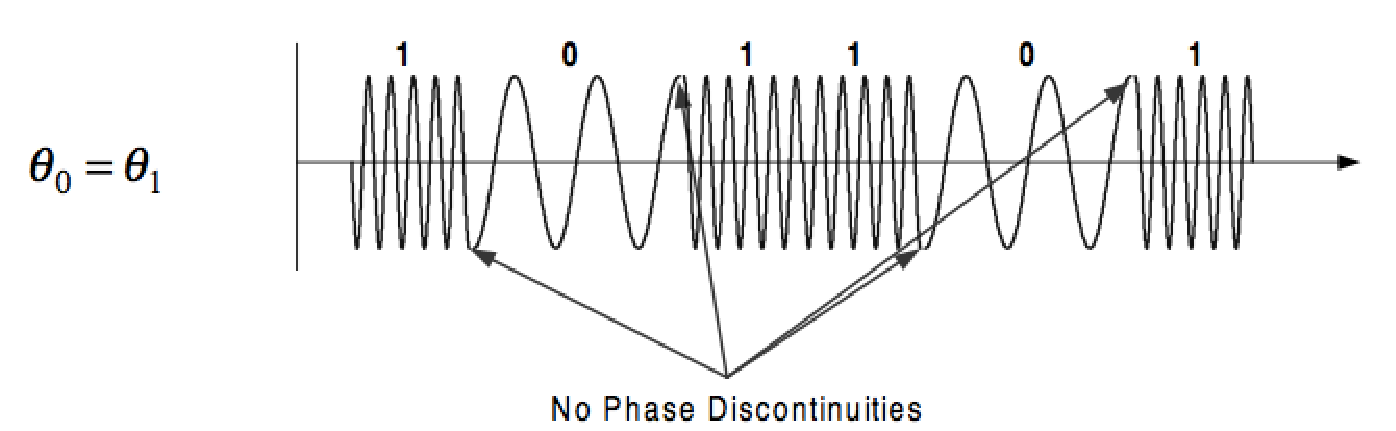
\includegraphics[width=0.6\textwidth]{cpfsk.pdf}
    \subcaption{Continuous phase FSK.}
    \label{fig:FSKnoncoherent}
 	\end{subfigure}
    \caption{FSK transmitted wave, with and without phase discontinuity\protect\cite{DigCommLec}.}
    \label{fig:comparecpfsk}
\end{figure}


\subsubsection{PSK}

Phase-shift keying (PSK)is a digital modulation scheme that conveys data by changing, or modulating, the phase of a carrier signal. A finite number of phases are assigned a unique pattern of binary digits. Usually,, each phase encodes an equal(even) number of bits. The demodulator, which is designed specifically for the symbol-set used by the modulator, determines the phase of the received signal and maps it back to the symbol that corresponds. In digital phase modulation, the M signal waveforms may be represented as: 
\[{s_i}(t) = A\cos ({\omega _c}t + {\phi _i}(t)) = \overbrace {A\cos ({\phi _i}(t))}^{inphase{\rm{ symbol }}{{\rm{x}}_i}(t)}*\cos ({\omega _c}t) + \underbrace {( - A\sin ({\phi _i}(t)))}_{{\rm{quadrature symbol }}{{\rm{x}}_q}(t)}*\sin ({\omega _c}t) = {x_i}(t)\cos ({\omega _c}t) + {x_q}(t)\sin ({\omega _c}t)\]

where $T_s$ is the symbol period, A the amplitude and M the number of points in the constellation diagram and the number of phases existing in the system. The decision regions for two different M-PSK schemes are depicted in figure \ref{fig:pskdr}.

 Alternatively, instead of using the bit patterns to set the phase of the wave, it can be used to change it by a specified amount. The demodulator then determines the changes in the phase of the received signal, rather than the phase itself. Since this scheme depends on the difference between successive phases, it is termed differential phase-shift keying (DPSK). 
 \begin{figure}[h]
  \centering
    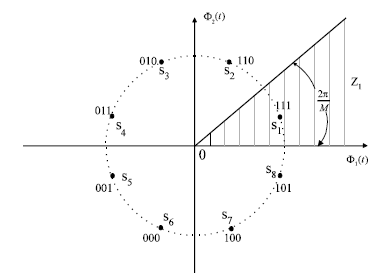
\includegraphics[width=0.7\textwidth]{PSKmodulation.png}
    \caption{Decision regions for 8-PSK. The minimum distance between symbols is given by $d_{min}=A\sin\frac{2\pi}{M}$ \cite{XiongDigModTech}.}
    \label{fig:pskdr}
\end{figure}

One of the advantages of PSK/DPSK is that it is more bandwidth efficient when compared to FSK. However, the signal detection/recovery is much harder when compared with ASK and FSK, since the demodulator must determine the phase of received sinusoid with respect to some reference phase. Additionally, if a higher rate PSK scheme is used, the equipment must be able to distinguish small differences in phase, making it unusable in time-varying channels. 



\subsection{Channel Equalization}
The performance of a digital system is limited by the type of channel in which the implementation is done. For our case, in theory, we have a nearly-ideal channel as we are working in the range of audible frequencies(up to 22.1 kHz). However, the phone's audio input and mic input introduce non-linear distortion that affects the signal output.
%Something about channel equalization in general, the method about how we do it should be in section METHOD

\subsection{Channel Coding}

The digital signal may be subject to diverse perturbations throughout a non-ideal channel and therefore, error correcting codes may be added. Our channel is bandwidth and power limited, these two parameters together with the noise spectral density will determine the bit-error rate (BER)\cite{HaykinBook}.In our system, the channel impairments result in frequency distortion and ISI. An orthogonal  modulation scheme may be able to mitigate such perturbations, however, it is still likely to have errors at the receiver that can be corrected by adding redundancy to the transmitted signal. This implies that the overall information rate will be decreased when using overheads such as training sequences or error correcting codes.
 
 There are two basic schemes to implement error correction capabilities into our system: error detection/retransmission, and forward error correction (FEC)\cite{SklarBook}. In the first scheme, the receiver terminal ask the transmitter to retransmit the data if it detects an error. For the case of using FEC, the receiver tries to recover the signal using the added redundancy. Hence, the detection and retransmission scheme requires a two-way communication contrary to the case of using forward error correction. We will focus on the last scheme since our system is only able to send data in one direction. In this fashion, the information message shall be encoded before it is modulated and sent trough the channel(figure \ref{fig:ChanCodTX}). The reverse process is done at the receiver, as shown in figure \ref{fig:ChanCodRX}.The most widely used codes are linear codes, which can be classified into two general forms: block codes, and convolutional codes. One of the principal differences between the two groups is that the encoder for the case of convolutional codes has memory elements.
 
  \begin{figure}[h]
  \centering
 	\begin{subfigure}[h]{0.9\textwidth}
  \centering
     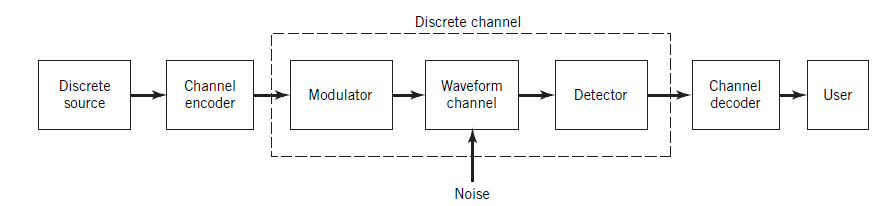
\includegraphics[width=0.6\textwidth]{chancodtx.png}
     \subcaption{Transmitter with channel encoder.}
     \label{fig:ChanCodTX}
 
 	\end{subfigure}
 	\quad
 
 	\begin{subfigure}[h]{0.9\textwidth}
  	\centering
     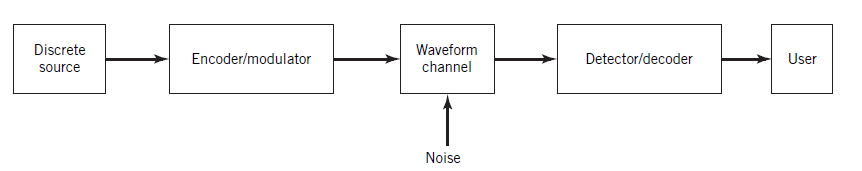
\includegraphics[width=0.6\textwidth]{chancodrx.png}
     \subcaption{Receiver with channel decoder.}
     \label{fig:ChanCodRX}
  	\end{subfigure}
     \caption{Scheme of a digital communication system with forward error correction \protect\cite{HaykinBook}.}
     \label{fig:ChanCoding}
 \end{figure}
 
 
 \subsubsection{Block Codes} 
 In general, binary block codes  are parity check codes that can be characterised by the parameters $(n,k)$. In this notation, $n$ represents the number of encoded bits, and $k$ is the number of information bits. We can define the ratio $k/n$ as the rate of the code. The mapping from the set of $M=2^k$ information sequences of length $k$ can be represented by a $k\times n$ generator matrix, conventionally denoted as $\bf{G}$. Therefore, we can write the encoded sequence $\bf{c}$ (of length $n$)in matrix form as follows:
\[{\bf{c}} ={{\bf{u}}}{\bf{G}}\]
The vector  $\bf{u}$ denotes the information sequence (of length $k$), and the row vectors of $\bf{G}$ determine the basis of a non-unique vector space. When $\bf{G}$ has the form ${\bf{G = }}\left[ {{{\bf{I}}_k}{\bf{|P}}} \right]$,
we can find out a parity matrix ${\bf{H = }}\left[ {{{\bf{I}}_{n - k}}{\bf{|}}{{\bf{P}}^T}} \right]$ that will enable us to decode back the original information\cite{SklarBook}. These codes are mainly used for hard-decision decoding with a built-in algebraic structure based in the properties of finite fields. There exist a variety of block codes termed as Long-Density Parity-Check Codes (LDPC) that can achieve performance very close to the channel capacity.  


 \subsubsection{Convolutional Codes}
 Convolutional codes are linear codes which are generated by passing the information sequence through a shift register. They can be described by some encoding function $G({\bf{u}})$ such that ${\bf{c}}=G({\bf{u}})$ The number of output bits for each $k$-bit input is a sequence of length $n$. We also need to define the parameter $K$ as the code constraint length, which represent the number of stages (of $k$-bits) in the encoder. 
Each path connecting the output to the input of a convolutional encoder can be characterised with the response of the encoder 
to the symbol 1 when each the shift registers are initialised to zero. The output is termed as the code's impulse response.

   

% % % % % % % % % % % % % % % % % % % % % % % % % % % % % % % % % % % % %
% % % % % % % % % % % % % % % % % % % % % % % % % % % % % % % % % % % % %


\section{Method}

In the last section, the fundamentals of each modulation scheme were introduced. Now we will focus on developing the details of the implemented modulation, demodulation and coding schemes. 

\subsection{MFSK}

FSK systems enjoy the highest power efficiencies among the available modulation schemes, but they are accompanied by the lowest bandwidth (BW) efficiency. In the following lines, we purpose a M-ary FSK system modulation scheme with orthogonal envelopes to improve the BW efficiency of the MFSK modulation. In M-ary FSK schemes, the modulated signals can be represented by:

\[{s_m}(t) = A{\varphi _m}(t),0 \le t \le T_s\],

where $T_s$ is the period of the input symbol stream and $A$ the amplitude of the basis function $\varphi_m$. This basis function can be described by:

\[{\varphi _m}(t) = \sqrt {\frac{2}{T}} \cos \left( {2\pi ({f_c} + {\alpha _m}\Delta {f_c}) + {\theta _m}} \right),0 \le t \le T\]


where \[{\alpha _m} \in \left\{ {(2m - 1 - M)|m = 1,2,...,M} \right\}\]. For orthogonality of the signals, the inner product between the basis functions must be 1 for $m=n$ and 0 for $m\neq n$, that is: 

\[\left\langle {\left. {{\varphi _m},{\varphi _n}} \right\rangle } \right. = \int {{\varphi _m}(t){\varphi _n}(t)dt = {\delta _{mn}} = \left\{ \begin{array}{l}
1,m = n\\
0,m \ne n
\end{array} \right.} \]


Individual frequencies corresponding to different symbols are given by \[{f_m} = {f_c} + {\alpha _m}\Delta {f_c}\], where $f_c$ is the central frequency and $\Delta f_c$ the frequency separation. In order to keep orthogonality, we must have \cite{gold}:

\[\Delta {f}= 2\Delta {f_c} = \left\{ \begin{array}{l}
\frac{1}{{2T}},{\theta _m} = {\theta _n},\forall m,n\\
\frac{1}{T},{\theta _m} \ne {\theta _n}
\end{array} \right.\]

The overall bandwidth occupied by the FSK signal depends on the modulation index $h=\frac{2\Delta {f_c}}{R}=2\Delta {f_c}T_s$. For continuous phase BFSK, the minimum value for the signals to not interfere with each other is $h=0.5$. Moreover, an FSK system using continuous phase transitions will have much lower side-lobe energy than the discontinuous case. All these parameters will hence affect the inter-symbol-interference (ISI) and limit the rate of the system. It is then important to further increase the bandwidth efficiency of the system by applying a pulse shaping function to the transmitted signal.

\subsection{Pulse Shaping Functions}

So far, we were considering the case where the signal is shaped by a rectangular function, inside the interval $0\leq t \leq T_s$. If $g(t)$, the pulse shaping function, is a rectangular pulse of width of $T_s$, then the envelope of the signal is constant. However, a rectangular pulse has very high spectral sidelobes, which means that signals must use a larger bandwidth to eliminate some of the adjacent channel sidelobe energy. Pulse-shaping is a method to reduce the sidelobe energy relative to a rectangular pulse, however the shaping must be done in such a way that ISI between pulses in the received signals is not introduced (or, at least, minimised). Assuming the channel model to be AWGN, the effective receive pulse is given by $p(t)=g(t) \ast c(t) \ast g^{*}(-t)=g(t) \ast g^{*}(-t)$, since the channel impulse response is given by $c(t)=\delta(t)$. This pulse must satisfy the Nyquist criterion, which requires the pulse to equal zero at the ideal sampling point associated with past or future symbols \cite{GoertzelPaper}: 

 \[p(k{T_s}) = \left\{ \begin{array}{l}
{p_0} = p(0),k = 0\\
0,k \ne 0
\end{array} \right.\]

Some of the pulses (also called windows) that satisfy this criterion are the rectangular, raised cosine (Hanning) and the root-raised cosine. Each pulse has advantages and disadvantages, but the last two are aimed to improve the spectral efficiency.The most common window in FSK is the Gaussian pulse defined as: 
 %This is nice, but I didn't found any space to put include it in this lines:---->
 %A mistiming error in sampling leads to a series of ISI components that converge. 
\[g(t) = \frac{{\sqrt \pi  }}{\alpha }{e^{ - {\pi ^2}{t^2}/{\alpha ^2}}}\]

where $\alpha$ is a parameter that dictates spectral efficiency. The spectrum of $g(t)$ is given by: 
\[G(f) = {e^{ - {\alpha ^2}{f^2}}}\]


The different windows characteristics can be seen in figure \ref{fig:wc} and their effect when applied to a simple BFSK system is depicted in figure \ref{fig:wcomp}. The parameter $\alpha$ in the gaussian window is related to the 3dB bandwidth of $g(t)$, $B_z$ \cite{GoertzelPaper}:
\[\alpha  = \frac{{\sqrt { - \ln \sqrt {0.5} } }}{{{B_z}}}\]

 \begin{figure}[h]
 \centering
  \label{fig:wincar}
\begin{subfigure}[h]{1\textwidth}
 \centering
    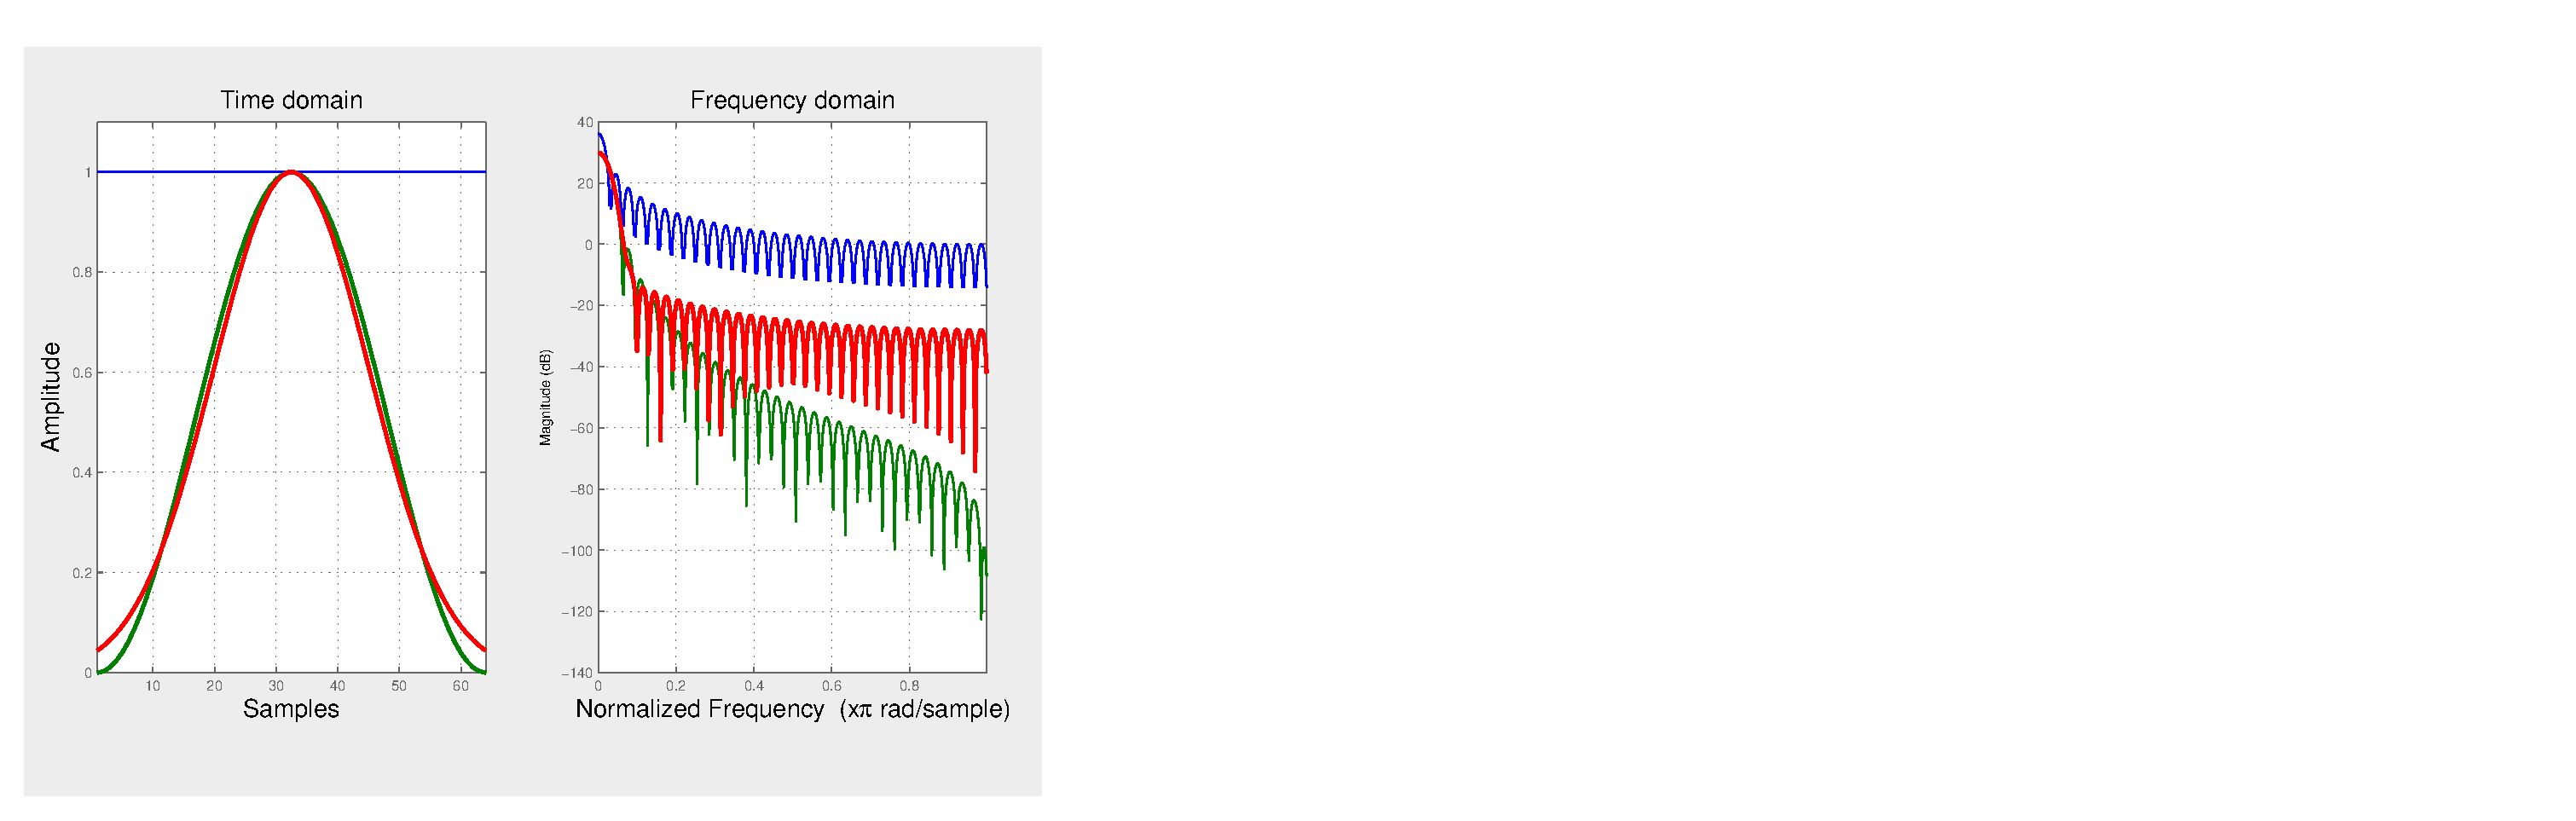
\includegraphics[scale=0.45, trim=0 0 30cm 0, clip=true]{wincomp.eps}
    \subcaption{Different windows in time and frequency domain. \textbf{Blue, red and green lines correspond to the rectangular, Gaussian and Hanning window, respectively.}}
    \label{fig:wc}
\end{subfigure}

\qquad
\qquad

\begin{subfigure}[h]{1\textwidth}
 \centering
    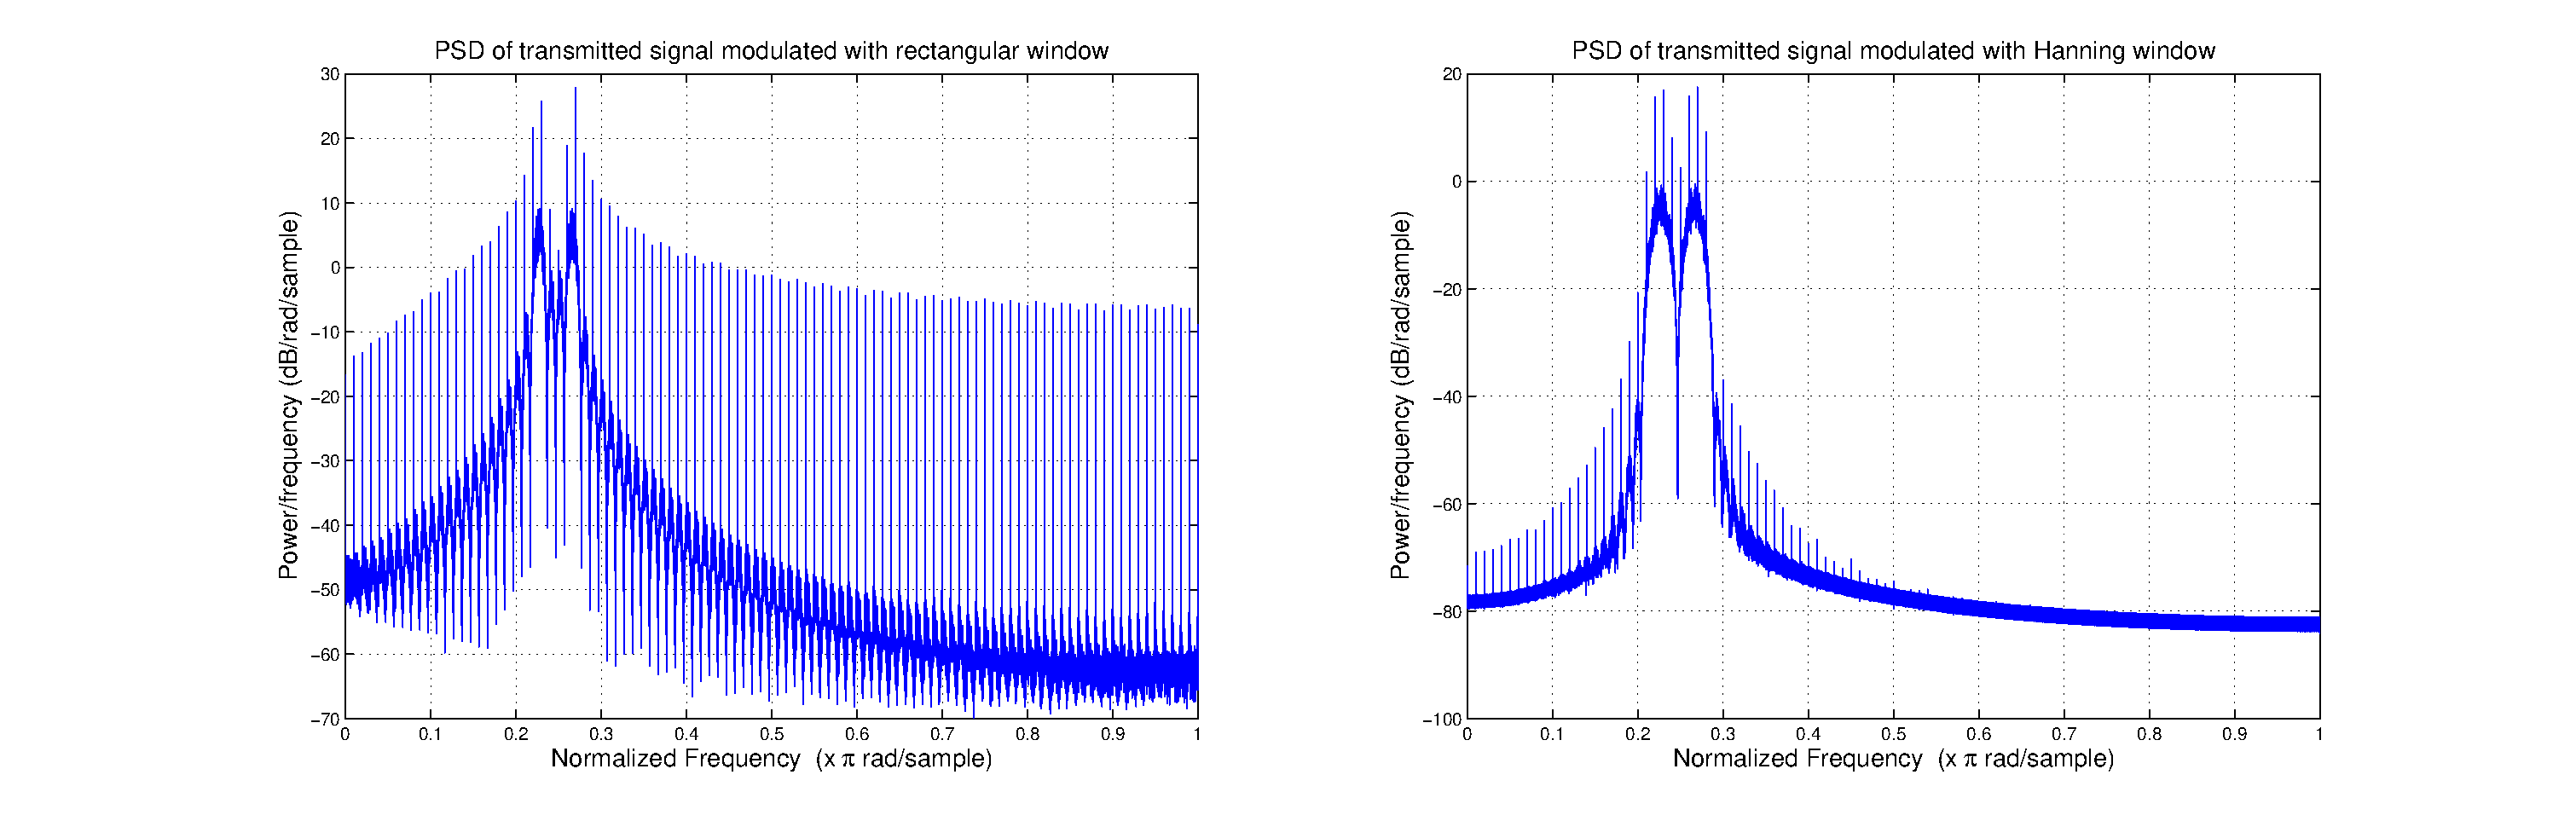
\includegraphics[scale=0.38]{txwinrectVShann.eps}
    \subcaption{PSD of the transmitted pulse using the rectangular and Hanning window for a BFSK system.}
    \label{fig:wcomp}
    
    \end{subfigure}
    
    \caption{The importance of choosing the right window for pulse shaping.}
    \label{fig:main}
\end{figure}

 Obviously, making $\alpha$ large results in a higher spectral efficiency. The Gaussian pulse does not satisfy the Nyquist criterion, and therefore the pulse shape introduces ISI, which increases as $\alpha$ increases. Therefore, improving spectral efficiency by increasing $\alpha$ leads to a higher ISI level, thereby creating an irreducible error floor from this self-interference. The variable $\alpha$ should, hence, be chosen with care. The gaussian window effect can be seen in figure \ref{fig:gaussianalpha} and will be further developed in the training sequence section \ref{subsec:ts}.

 \begin{figure}[h]
  \centering
    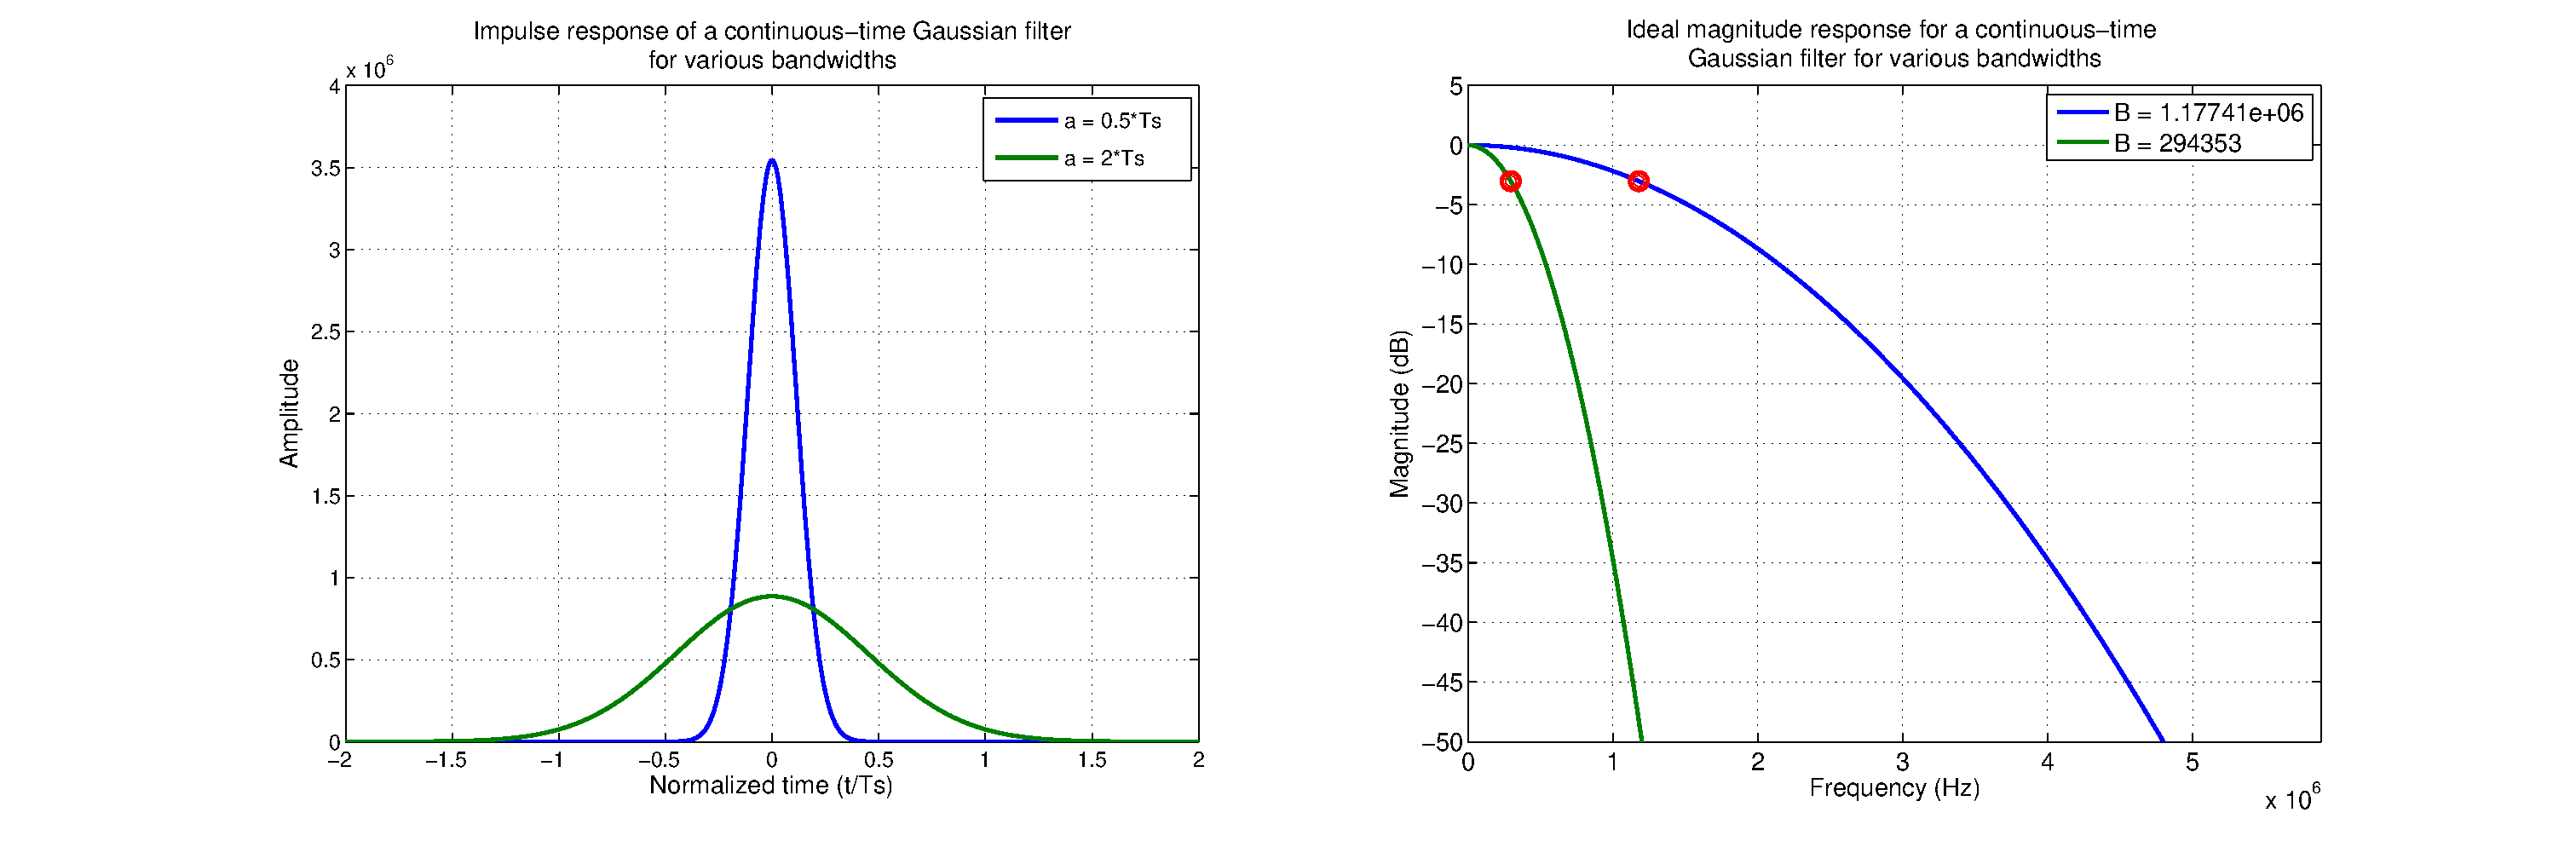
\includegraphics[width=1\textwidth]{gausswinalpha.eps}
    \caption{Ideal Gaussian filter with different values of $\alpha$. The tradeoff between high spectral efficiency and reduced ISI is clear. A large $\alpha$ leads to an increased efficiency but the amplitude for $t/T_s > 1$ is not zero, leading to ISI.}
    \label{fig:gaussianalpha}
\end{figure} 
 

\subsection{Efficient MFSK Demodulation}

The demodulators presented in part \ref{subsec:fsk} are interesting from a theory point of view. However, for real time, software-based applications there are other methods for efficient demodulation. One of these methods is the Discrete Fourier Transform (DFT) which evaluates the amplitude and phase for each frequency present in the received signal. Since we are using a MFSK modulation scheme, a tone/frequency detector such as DFT for a symbol period is a powerful tool for a correct and efficient demodulation. However, we are only interested in detecting one or more tones in an audio signal and at the same time we are constrained to the CPU horsepower provided by the smartphone. Taking this into account, we purpose a much faster method, when compared with FFT for instance, which is the Goertzel algorithm. 

\subsection{Goertzel Algorithm}
\label{sec:FSKdemod}
%Add a reference of a publicationr related with Goertzel's Algorithm
There are various ways to detect the presence of a special known frequency in a received signal. The DFT algorithm is a simplistic way to check whether the desired frequency is present and a FFT produces the same numerical result for a single frequency of interest, making it a better choice for tone detection. The Goertzel algorithm is a DFT in disguise, with some numerical tricks to eliminate complex number arithmetic, increasing the efficiency over the FFT under some constraints. This section aims to present the Goertzel algorithm.

The idea is to transform an ordinary N samples DFT into a Goertzel filter form. Defining $W_{N}^{k}={e^{ - j2\pi k/N}}$ and noting that ${W_N}^{ - Nk} = 1$, we have for the DFT \cite{GoertzelPaper}:
\[X(k) = \sum\limits_{n = 0}^{N - 1} {x(n){W^{nk}}_N}  = \sum\limits_{n = 0}^{N - 1} {x(n){W_N}^{ - Nk}{W^{nk}}_N}  = \sum\limits_{n = 0}^{N - 1} {x(n){W_N}^{ - (N - n)k}} \]
An efficient way to evaluate this polynomial is the nested form:
\[X(k)=\bigg(\big(({W^{ - k}_N}x(0) + x(1)\big){W_N}^{ - k} + x(2)){W_N}^{ - k} + ... + x(N - 1)\bigg){W_N}^{ - k}\]

The last expression can be written in terms of a recursive difference equation:
\[y(n) = {W^{ - k}_N}y(n - 1) + x(n)\]

Expressing the difference equation in the z-transform domain and by multiplying both numerator and denominator by (${1 - {W_N}^{ - k}{z^{ - 1}}}$), we get the transfer function:

\[\frac{{Y(z)}}{{X(z)}} = H(z) = \frac{1}{{1 - {W_N}^{ - k}{z^{ - 1}}}} = \frac{{1 - {W_N}^{ - k}{z^{ - 1}}}}{{1 - (2\cos (\frac{{2\pi k}}{N}){z^{ - 1}} - {z^{ - 2}})}}\]

The Goertzel algorithm acts as an IIR filter that uses the feedback path to generate a very high Q bandpass filter, where the coefficients are easily generated from the required center frequency.  It is mostly implemented as the second order recursive IIR filter, as shown in figure \ref{fig:IIR}. 
 \begin{figure}[h]
  \centering
    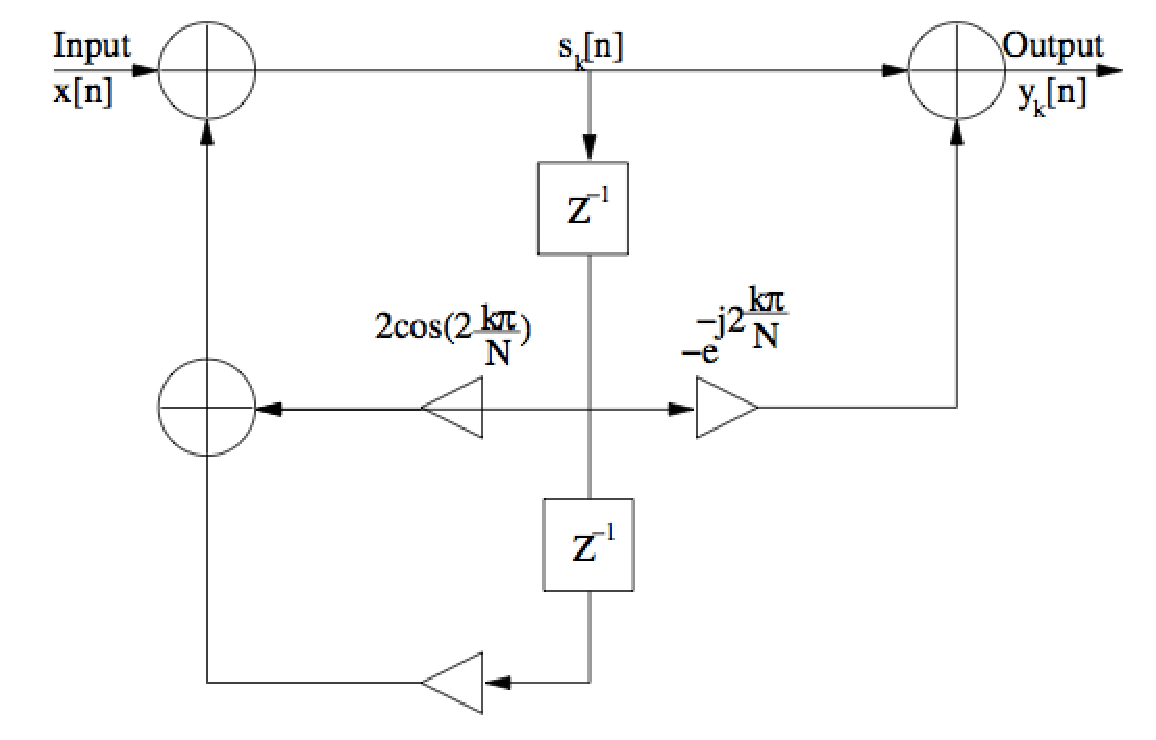
\includegraphics[width=0.5\textwidth]{IIR.pdf}
    \caption{Direct-Form Realisation of the Goertzel Algorithm \protect\cite{HaykinBook}.}
    \label{fig:IIR}
\end{figure}


The algorithm computes the k-th DFT coefficient $X(k)=y(N)$ of the input signal $x(n)$ using the 2nd order filter:
\begin{equation}
\begin{array}{l}
{s_k}(n) = x(n) + 2\cos (\frac{{2k\pi }}{N}){s_k}(n - 1) - {s_k}(n - 2)\\
{y_k}(n) = {s_k}(n) - {W_N}^k{s_k}(n - 1)
\end{array}
\label{fig:IIRtime}
\end{equation}

with ${s_k}( - 1) = {s_k}( - 2) = 0$. The discrete frequencies in which the algorithm is able to compute the DFT are ${f_k} = \frac{k}{N}{f_s}$ for $f \leq \frac{f_s}{2}$.
%%The computation for $s_k(n)$ takes one add ($x(n)-s_k(n-1)$) and one %%multiply-accumulate per received sample.

\subsubsection{Computational and Memory complexities}

The FFT algorithm used with N being a power of two has computational demands proportional to $\mathcal{O}(N\log_2 N)$. The absolute number depends on the particular implementation. Usually the number of real-number arithmetic operations found in the literature is approximately $6N \log_2 N$. If we analyse the number of operations of the Goertzel algorithm, we realize that for a real input signal, $N$ real multiplications and $2N$ real additions are performed and, hence, $3N$ operations for a single frequency. Ignoring the computations of the cosine and the exponential constants in equation \ref{fig:IIRtime}, then if N frequencies would be of interest, the Goertzel algorithm would be of quadratic complexity as the DFT is. To answer the question for how many frequencies $K$ is it more advantageous to exploit the Goertzel algorithm than the FFT, we compare and conclude that \cite{GoertzelPaper}: 
\begin{equation}
3NK < 6N{\log _2}N \Leftrightarrow K < 2{\log _2}N
\label{eq:ineffgor}
\end{equation}

Such a result, however, holds only for N being a power of two; otherwise the inequality \ref{eq:ineffgor} can even be more favourable for the Goertzel algorithm.

Considering real inputs solely, the FFT algorithm requires a memory space of at least $2N$. Also, the $n$ values of the transformation kernel, $sin$ and $cos$, are often precomputed and stored. The FFT calculation itself can be performed with no values being moved in memory, but as the computation cannot be done until the last sample of a block of data is received, a buffer size of at least $N$ must be used. Therefore, the overall FFT memory demand is $4N$ for real signals.
For each considered frequency, the Goertzel algorithm requires: location for saving one real and one complex state variable, the complex final output and the last 2 real outputs $s_k(n) and s_k(n-1)$. There is no need to implement input buffering, because the computation can be run as the new signal samples arrive. The total memory complexity of the Goertzel algorithm is thus $7K$ positions. Combining all the above together, the Goertzel algorithm will be less memory-demanding than the FFT if \cite{GoertzelPaper}
\[7K < 4N \Leftrightarrow K < \frac{4}{7}N\]

As long as $N\geq 13$ equation \ref{eq:ineffgor} is decisive for choosing the best algorithm since for these N it holds that $\frac{4}{7} N \leq 2 \log_2 N$.

\subsection{Synchronisation}
\label{subsec:ts}
Up to this point we have assumed that the receiver is perfectly synchronised with the transmitter and the only channel impairment is AWGN. In practice, however, it is often found that there is also uncertainty due to the randomness of some signal parameters, caused by distortion in the transmission medium. Perhaps the most common random signal parameter is the carrier phase, which is especially true for narrowband signals. 

There are two basic modes of synchronisation in the reception of a digitally modulated signal:
\begin{enumerate}
%Paraphrase the following line:
\item \textbf{Carrier Synchronisation}  When coherent detection is used in signalling via the modulation of a sinusoidal carrier, knowledge of both  
frequency and phase of the carrier are necessary. 
The process of estimating the carrier phase and frequency is called carrier recovery. 

\item \textbf{Clock recovery} To perform demodulation, the receiver has to know the instants of time that at which the modulation in the transmitter changes its state. In other words, the receiver has to know the starting and finishing point of the individual symbols, so that it may determine when to sample. The estimation of these times is called symbol synchronisation.
\end{enumerate}


\subsubsection{Symbol Synchronisation}
The synchronisation algorithm is crucial for the operation of the system. Its task is to find the best sampling time for the sampling device. Ideally, the MF should be sampled such that the SNR for the decision variable is maximised. For a rectangular pulse shape, the best sampling time $t_{samp}$ is at the peaks coming out from the matched filter (see figure \ref{fig:mfpeaks}).

 \begin{figure}[h]
  \centering
    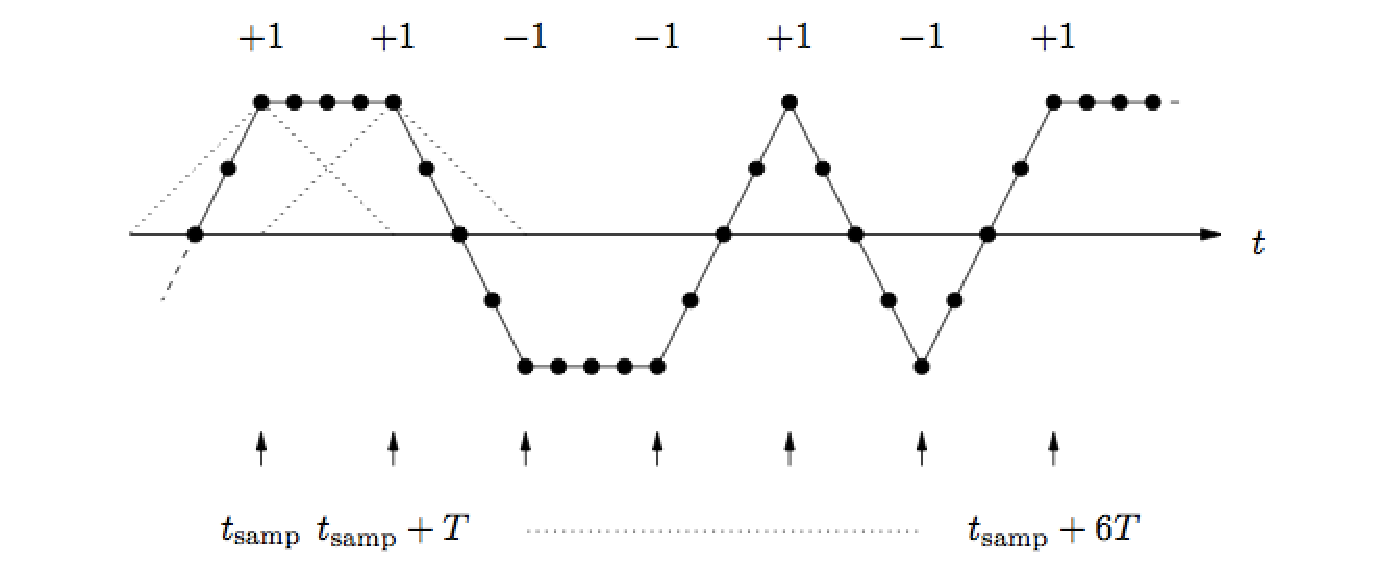
\includegraphics[width=0.7\textwidth]{mfpeaks.pdf}
    \caption{Output from the matched filter for successive signalling in absence of noise. The small arrows illustrate the preferred sampling instants\protect\cite{ProjectEQ2310}.}
    \label{fig:mfpeaks}
\end{figure}


The used algorithm is based on the training sequence. During the training sequence, it is know to the receiver what the transmitter is transmitting. Hence, one possible way of recovering the symbol time is to cross-correlate the samples after the matched filter with a locally generated time-shifted replica of the training sequence. This algorithm can be either applied directly to the received samples and correlating with a modulated training sequence (resolution of 1 sample but very sensitive) or applied at the symbol level (resolution of $\frac{T}{Q}$, where Q is the number of samples per symbol). Let's consider the last option for simplifying purposes. If ${\left\{ {c(n)} \right\}_{n = 0}^{L - 1}}$ is the locally generated symbol-spaced replica of the training sequence of length L, [$t_{start},t_{end}$] represents the search window and $r(n)$ denotes the output from the matched filter, the timing can be found as \cite{HaykinBook}:

\[{t_{samp}} = \arg \mathop {\max }\limits_{{t_{samp}} \in [{t_{start}},{t_{end}}]} \left| {\sum\limits_{k = 0}^{L - 1} {r(kQ + {t_{samp}})^*c(k)} } \right|\]


The correlation properties of the training sequence are important as they affect the estimation accuracy. Ideally, the autocorrelation function for the training sequence should equal a delta pulse, i.e., zero correlation everywhere except at lag zero. Therefore, the training sequence should be carefully designed. If, for example, the training sequence is modulated with a different frequency or a different pulse shape is used, from the rest of the signal, better results for the correlation are obtained, as can be seen in figure \ref{fig:tscomp}. 

\begin{figure}[h] 
  \begin{subfigure}[b]{0.5\linewidth}
    \centering
    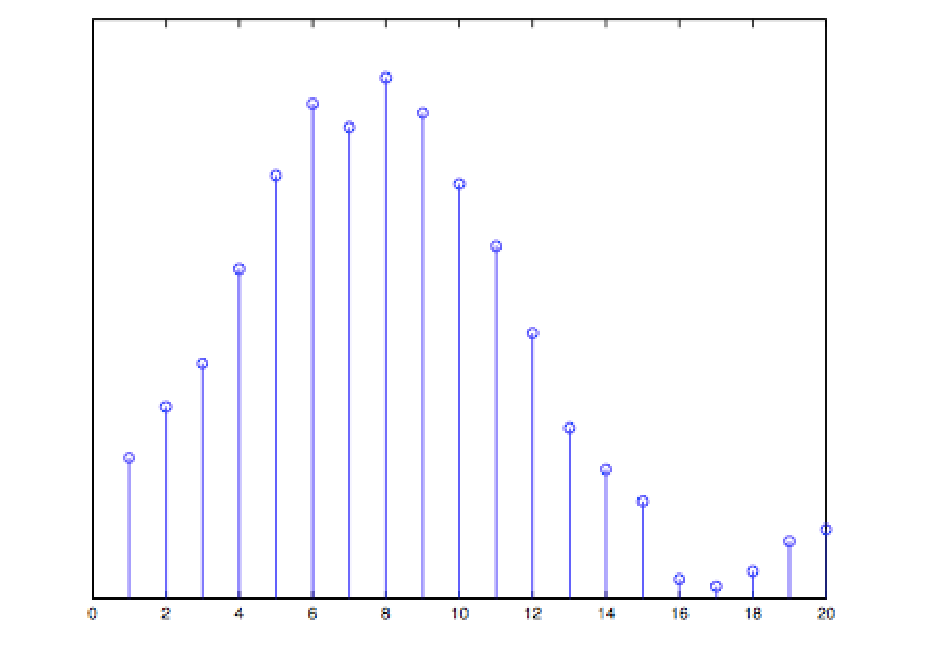
\includegraphics[width=1\linewidth]{ss.pdf} 
    \caption{Symbol spaced cross-correlation. In this example the delay is estimated to be 8 and therefore the system should be sampled at 8+kQ, k=0,1,2,..N.} 
    \label{fig:a} 
    \vspace{4ex}
  \end{subfigure}%% 
  \quad
  \begin{subfigure}[b]{0.5\linewidth}
    \centering
    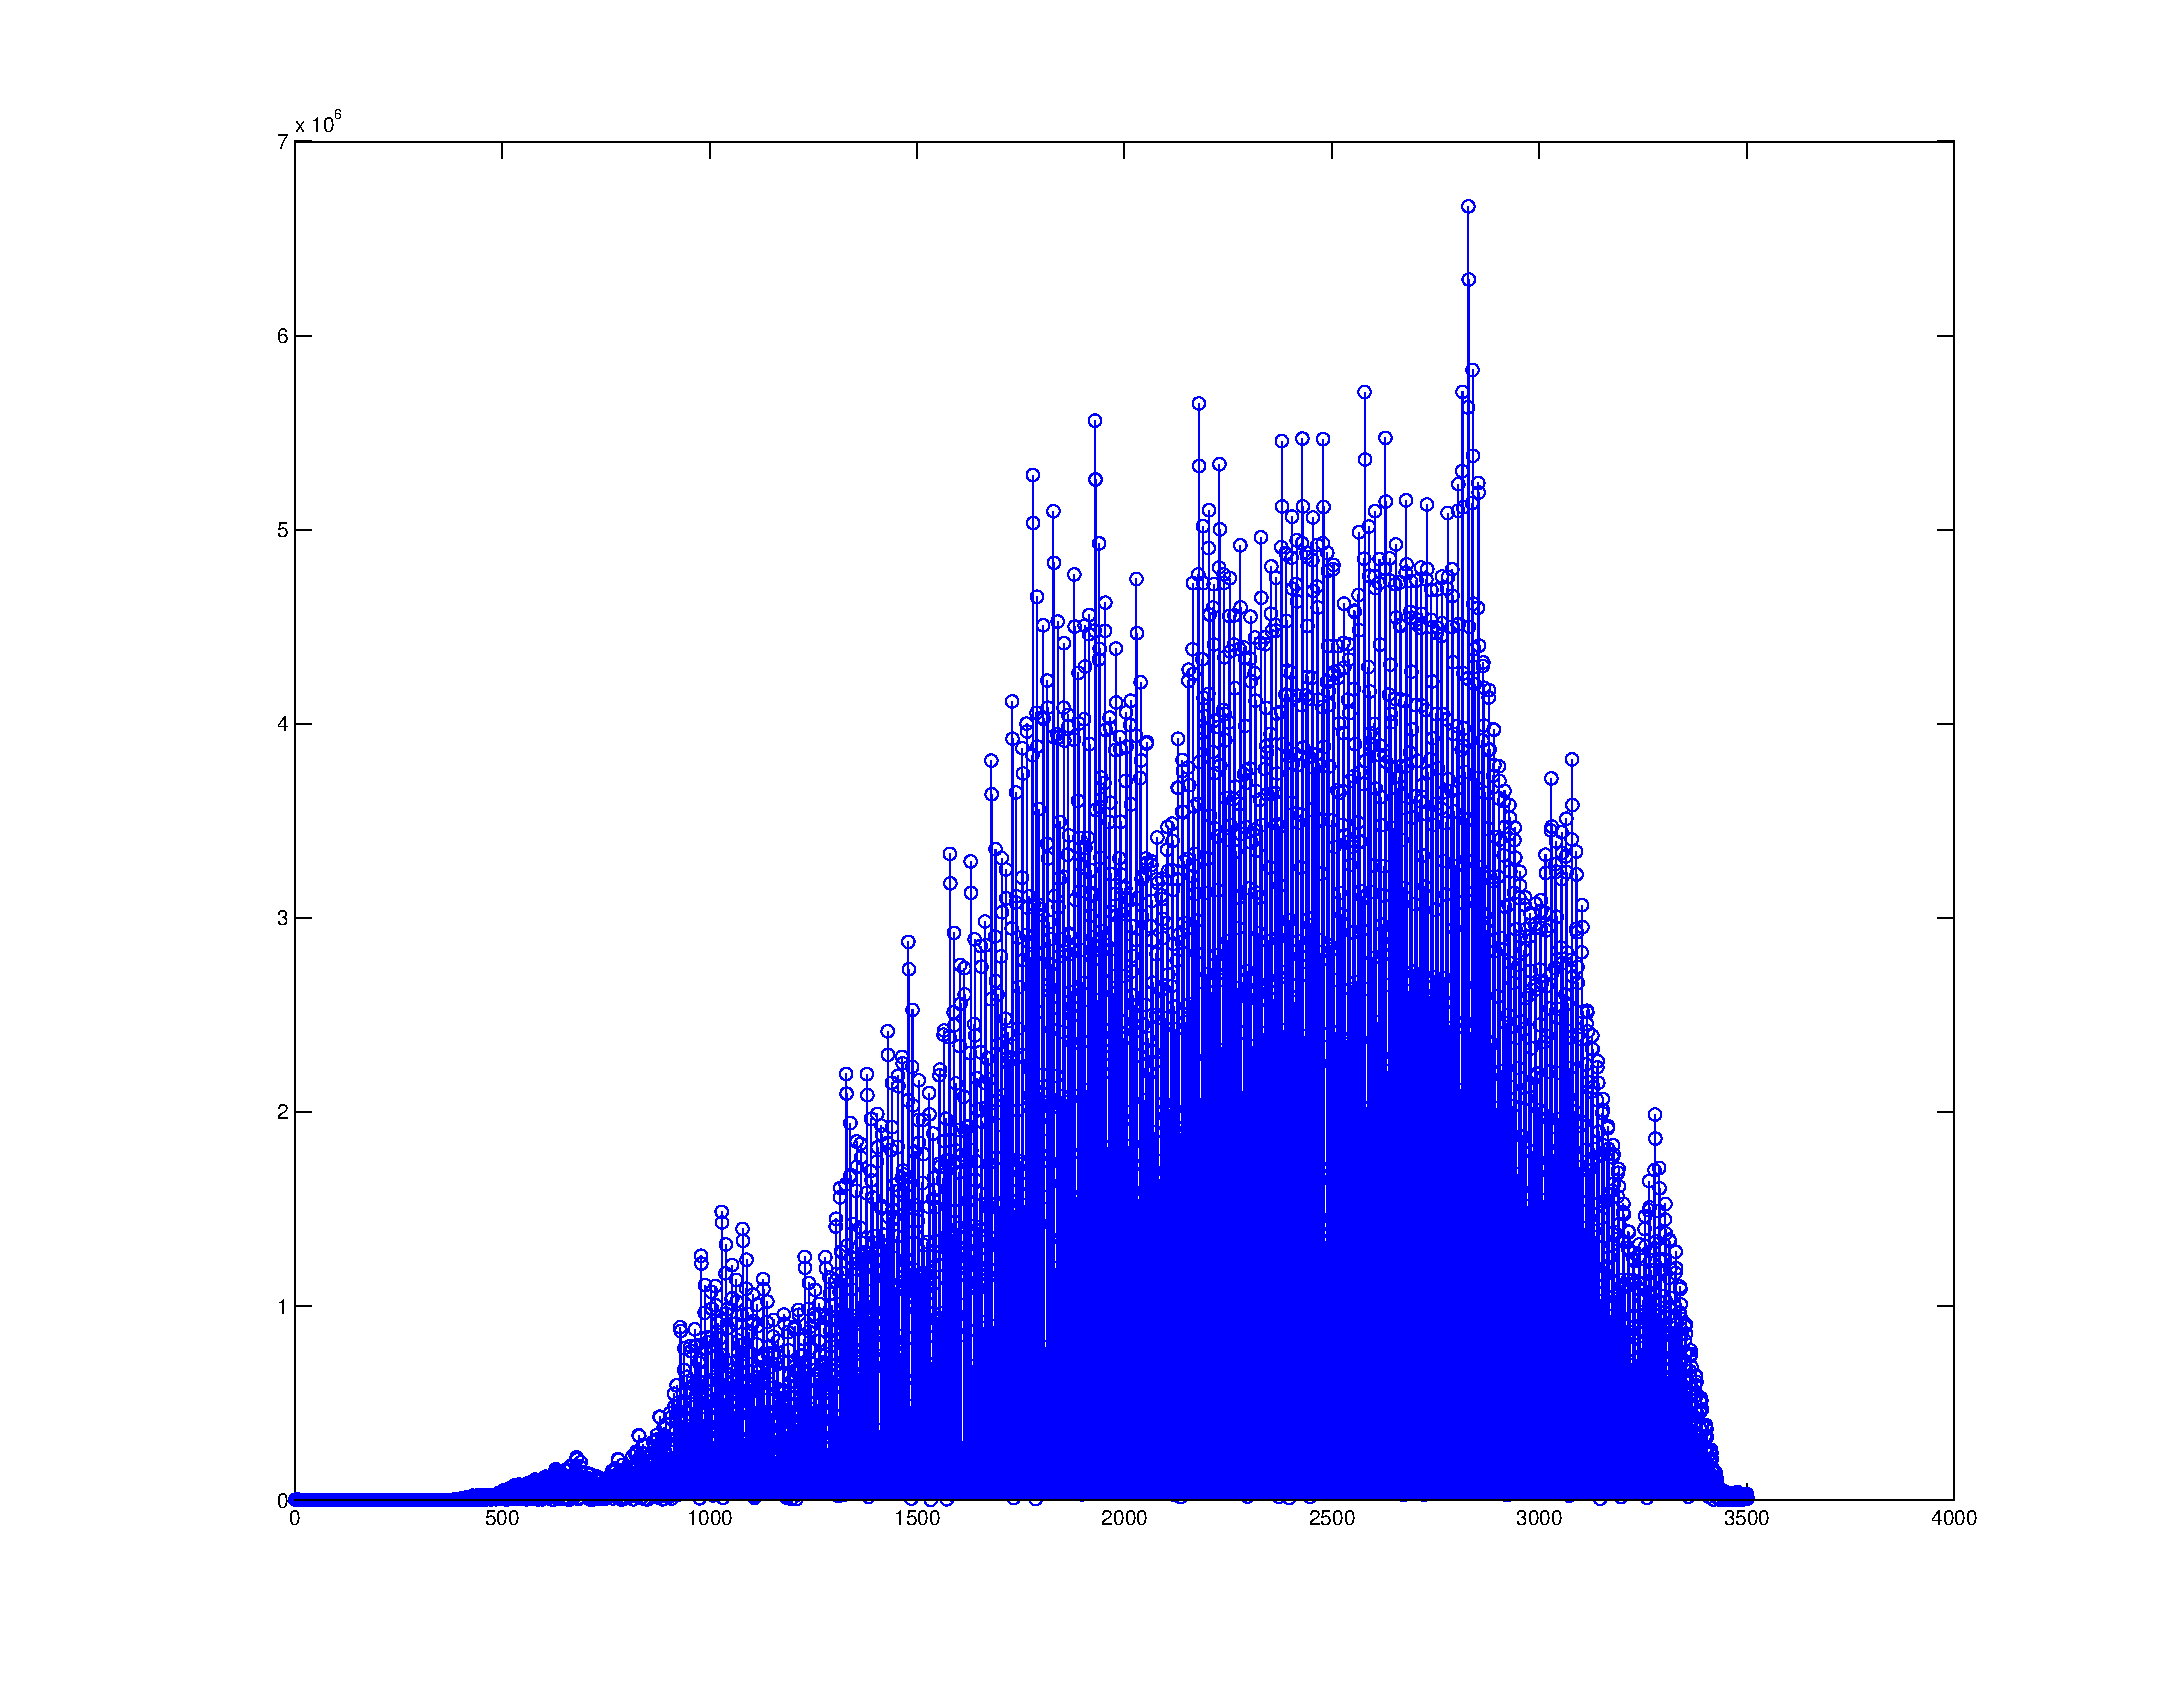
\includegraphics[width=1\linewidth]{20.eps} 
    \caption{One sample resolution cross correlation with training sequence of length 20 symbols.} 
    \label{fig7:b} 
    \vspace{4ex}
  \end{subfigure} 
  \quad
  \begin{subfigure}[b]{0.5\linewidth}
    \centering
    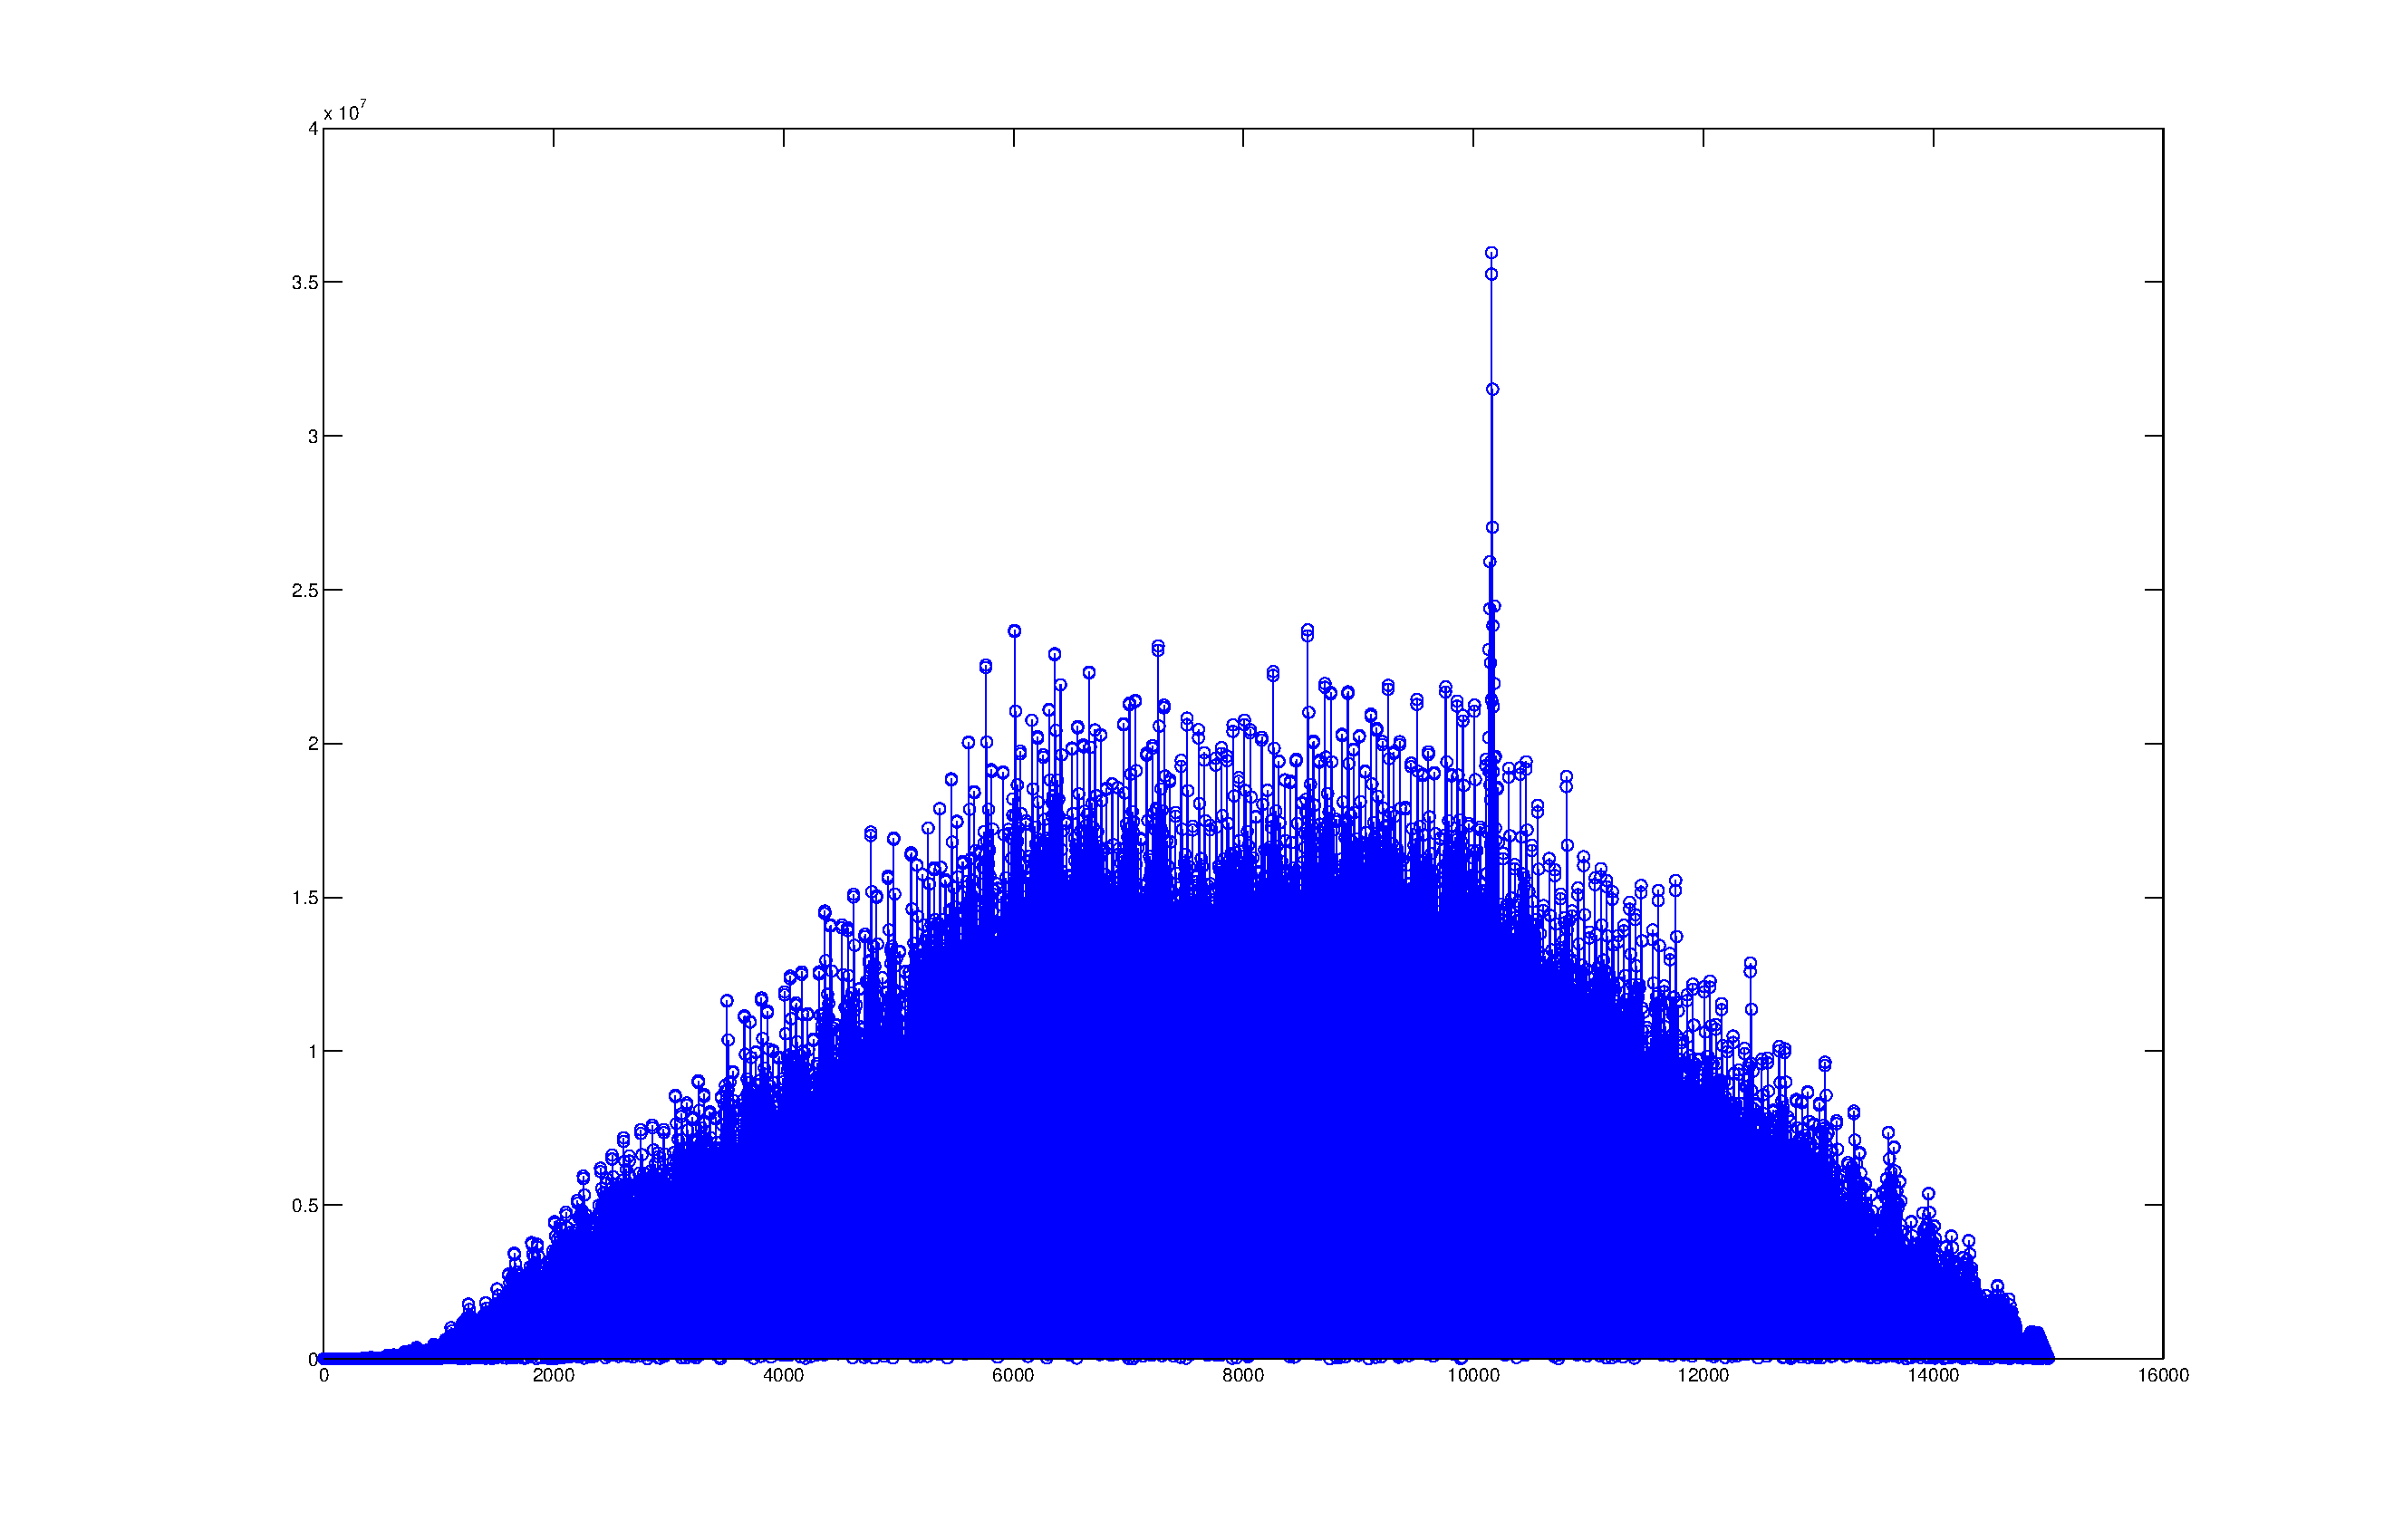
\includegraphics[width=1\linewidth]{100eq.eps} 
    \caption{One sample resolution cross correlation with training sequence of length 100 symbols and equal frequency to rest of trasmission.} 
    \label{fig7:c} 
  \end{subfigure}%%
  \quad
  \begin{subfigure}[b]{0.5\linewidth}
    \centering
    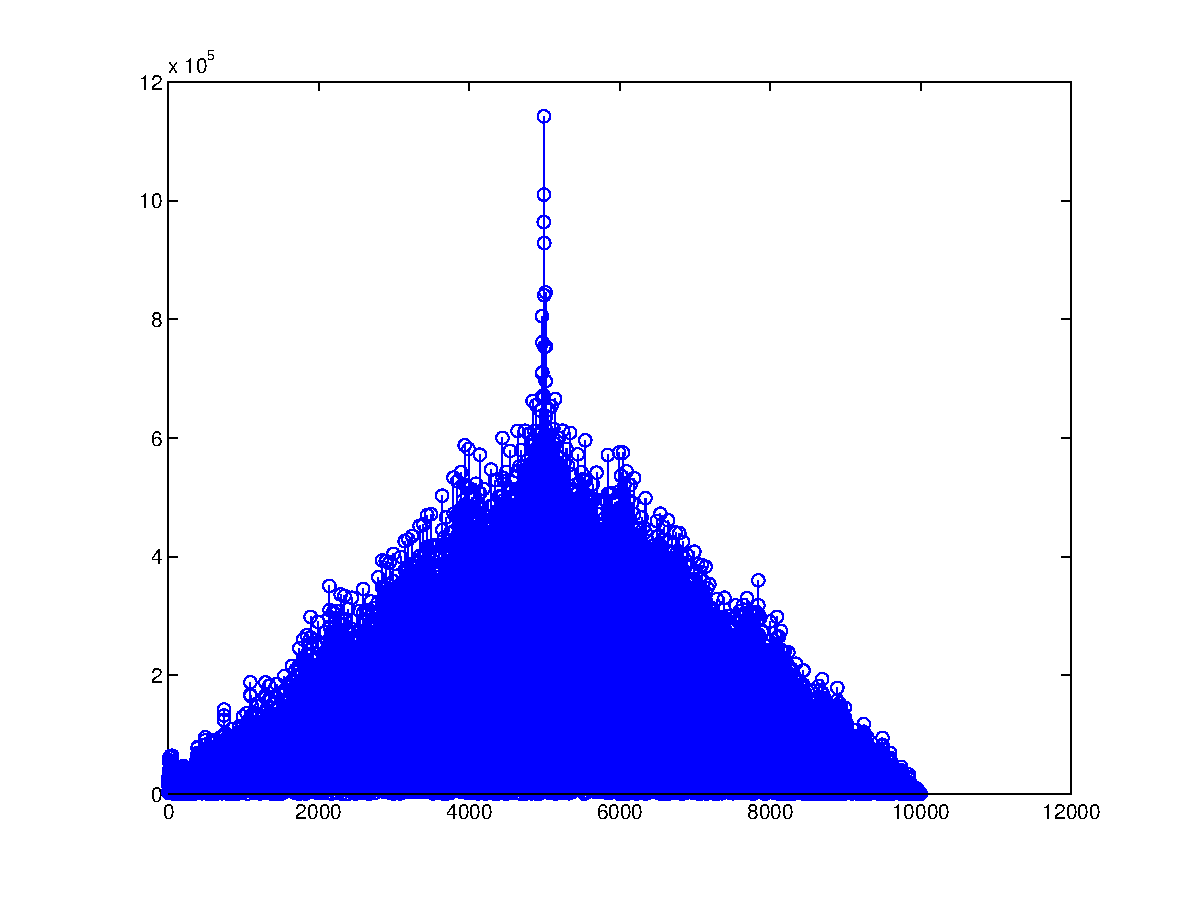
\includegraphics[width=1\linewidth]{100dif.eps} 
    \caption{One sample resolution cross correlation with training sequence of length 100 symbols and different frequency to rest of transmission.} 
    \label{fig7:d} 
  \end{subfigure} 
  \caption{Training sequence algorithm/length/modulation comparison.}
  \label{fig:tscomp} 
\end{figure}
   
\subsubsection{Carrier Synchronisation}

The basic operations required by an all digital MQAM receiver are illustrated in figure \ref{fig:rxMQAM}. The quadrature down-conversion and matched filter operations produce estimates of the quadrature amplitudes that are the basis of the data decisions. The role of carrier phase synchronisation is to perform the quadrature down-conversion using phase coherent replicas of the quadrature carriers.

 \begin{figure}[h]
  \centering
    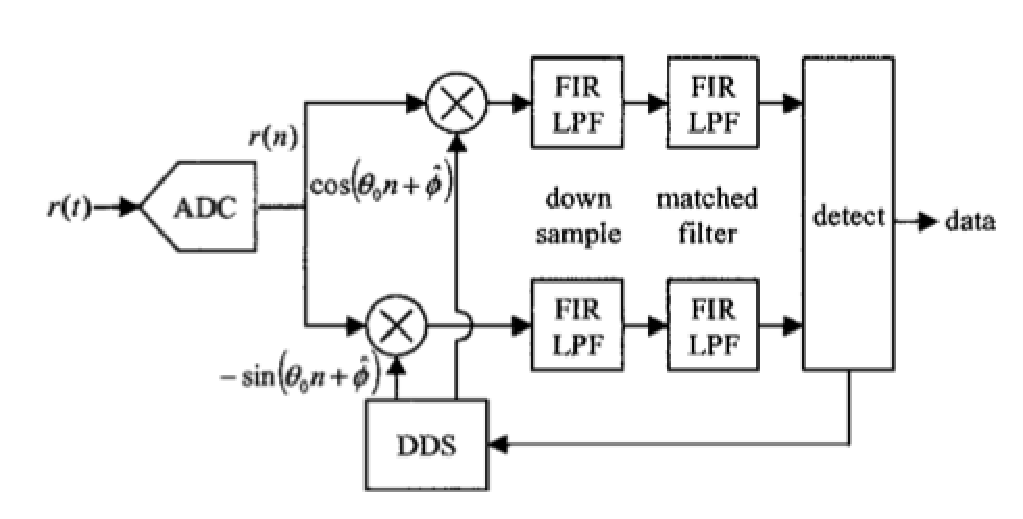
\includegraphics[width=0.6\textwidth]{rxMQAM.pdf}
    \caption{Block diagram of basic QPSK/QAM digital receiver. In the digital implementation, the VCO takes the form of a direct digital synthesizer (DDS). }
    \label{fig:rxMQAM}
\end{figure}

There are many options for implementing carrier phase and frequency synchronisation in a digital communication system. At the heart of all synchronisers is the phase-locked loop (PLL). An all-digital receiver can be implemented with a digital phase-locked loop (DPLL) as shown in figure \ref{fig:DPLL}. The phase detector is implemented using the arctangent suggested by the ATAN block. The complexity of the phase detector can be reduced by computing a signal proportional to the sine of the phase difference. The phase error is computed by comparing the phase difference between the received signal $x(n) + jy(n)$ and the closest constellation point $\hat{I}(n) + j\hat{Q(n)}$ as illustrated in figure \ref{fig:PD1}.

 \begin{figure}[h]
 \centering
\begin{subfigure}{0.5\textwidth}
 \centering
    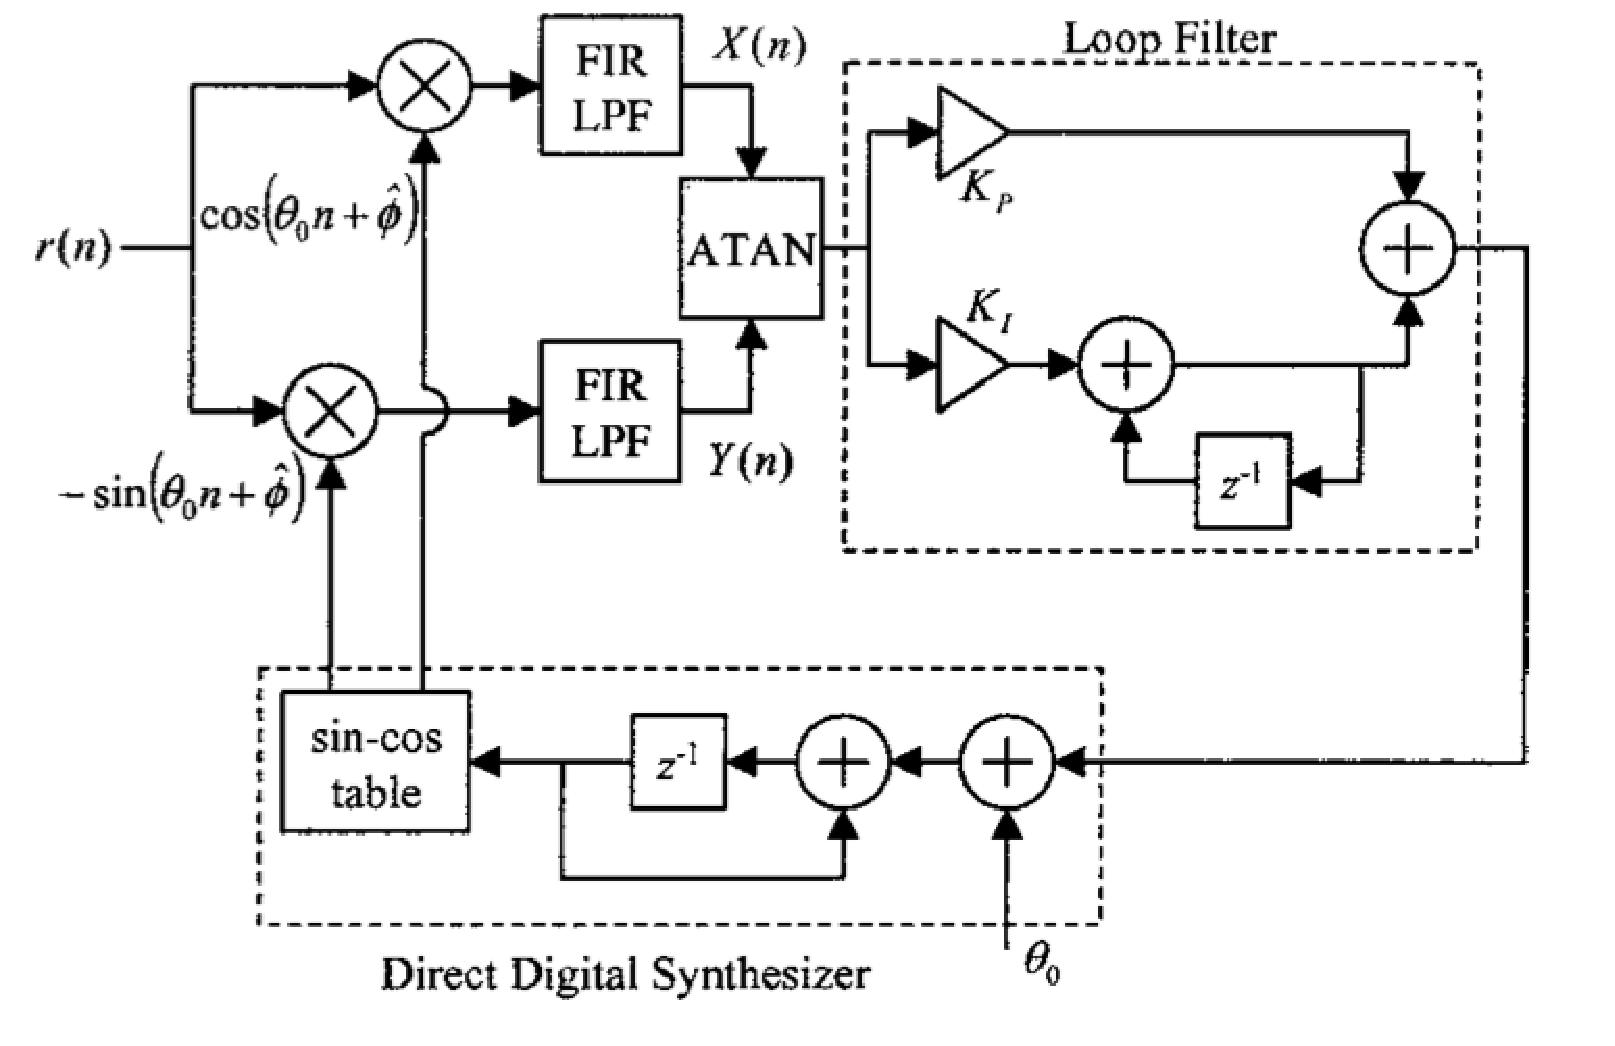
\includegraphics[width=0.9\linewidth]{DPLL.pdf}
    \caption{Digital phase locked loop for carrier phase synchronisation.}
    \label{fig:DPLL}
\end{subfigure}%
\begin{subfigure}{0.5\textwidth}
 \centering
    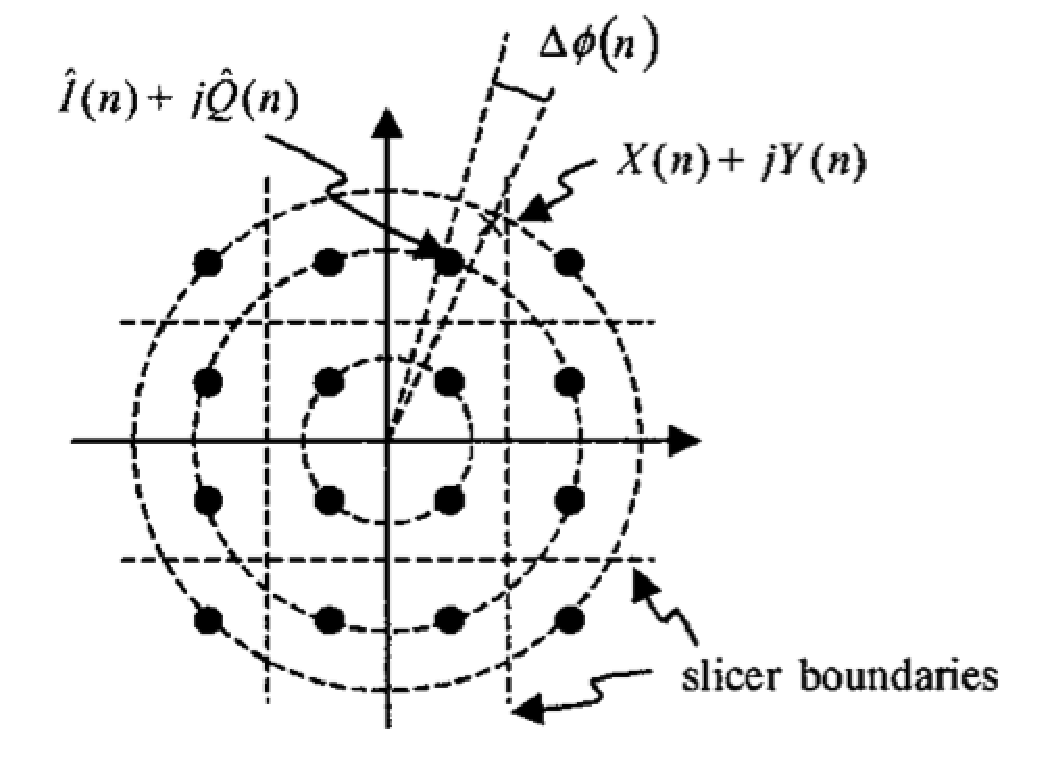
\includegraphics[width=0.7\linewidth]{PD.pdf}
    \caption{16-QAM constellation with decision boundaries and phase error.}
    \label{fig:PD1}
    \end{subfigure}
    \caption{Carrier phase estimation diagrams\protect\label{CarrierSynchPaper}.}
    \label{fig:carrierphase}
\end{figure}



The initial phase estimation can be done using the above procedure, taking into account the training sequence is known at transmitter and receiver. Let's assume the channel causes a rotation of $\varphi$ to the symbol constellation. The value of $\varphi$ can be computed using the element-wise multiplication of the received symbol with the complex conjugate of a modulated training sequence replica and then averaging over the sequence. In other words, if ${\left\{ {\tilde r(n)} \right\}_{n = 0}^{L - 1}}$ denotes the L received symbols and ${\left\{ {c(n)} \right\}_{n = 0}^{L - 1}}$ the local replica of the complex training sequence, an estimate of the phase offset can be obtained as \cite{ProjectEQ2310}:
\[\hat \varphi  = \frac{1}{L}\sum\limits_{k=0}^{L - 1} {\arg (\tilde r(k)c(k)^*)} \]
The longer the training sequence, the better the phase estimate as the influence from the noise decreases. A long training sequence, on the other hand, reduces the amount of payload that can be transmitted during a given time.

Another problem that may be faced in a real implementation is the Doppler shift introduced during the transmission, which causes the constellation to rotate further more (than the initial rotation). This frequency offset could be the result of relative motion between the transmitter and receiver, as would be the case with a mobile terminal travelling away or towards a receiver. It could also be attributed to small frequency variations of the various synthesisers in both the transmitter and receiver, which are functions of time and temperature. In order to overcome this problem, at least two approaches are possible. The first is to introduce a training sequence in the data so that a new phase estimation can be computed, resulting in a lower rate. The other solution, is to divide the decisions into various small blocks in which the offset does not influence the decision, estimate the phase rotation from the nearest points and rotate the constellation for future decisions. In this way, the rate is not affected but a correct decision in each block is assumed. The frequency offset effect can be seen in figure \ref{fig:phaseoff}, where a signal of 5 seconds was transmitted. The second solution was used to correct the phase with great success.


 \begin{figure}[h]
 \centering
\begin{subfigure}{0.32\textwidth}
 \centering
    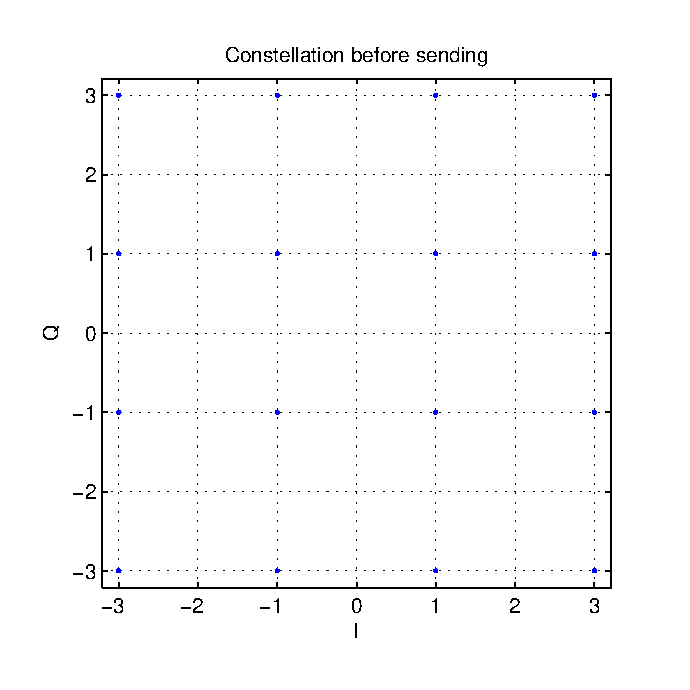
\includegraphics[width=0.8\linewidth]{tx_const.eps}
    \caption{Transmitted constellation.}
    \label{fig:DPLL2}
\end{subfigure}%
\begin{subfigure}{0.32\textwidth}
 \centering
    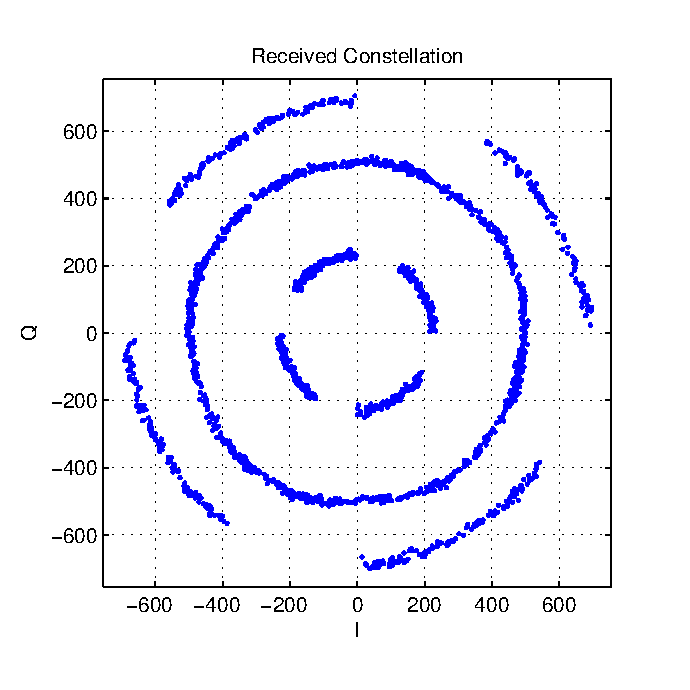
\includegraphics[width=0.8\linewidth]{rx_const.eps}
    \caption{Received constellation.}
    \label{fig:PD2}
    \end{subfigure}
    \begin{subfigure}{0.32\textwidth}
 \centering
    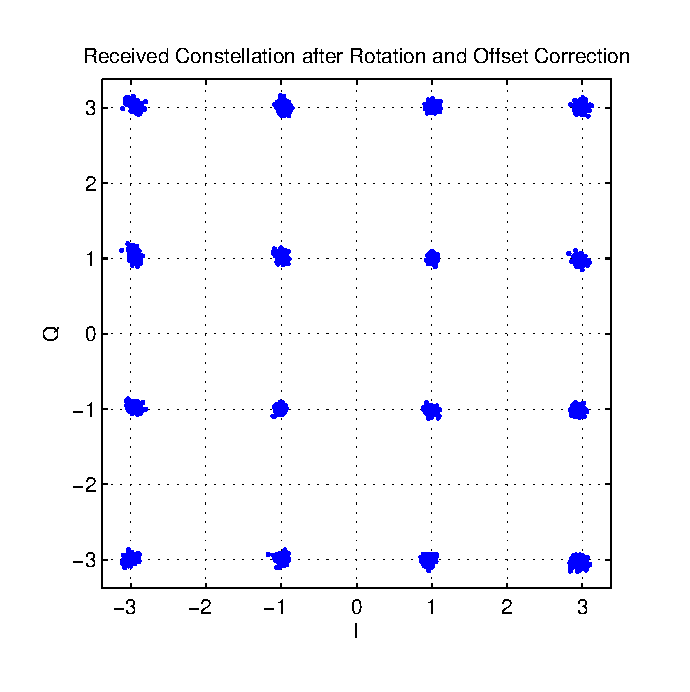
\includegraphics[width=0.8\linewidth]{rx_const_after.eps}
    \caption{Received constellation after phase correction.}
    \label{fig:PD3}
    \end{subfigure}
    \caption{Example of frequency offset in a 16-QAM constellation with decision boundaries.  }
    \label{fig:phaseoff}
\end{figure}

%By trying different time-shifts in steps of $\frac{T}{Q}$, where Q is the number of samples per symbol, the symbol timing can be found with a resolution of  $\frac{T}{Q}$.  

\clearpage


\subsection{Channel Coding}
Since our system will be implemented mostly in software, we should come up with a coding scheme that does not introduce too much delay and heavy processing to the phone. On the other hand, our goal is to implement an application capable to transmit digital files, thereby we should guarantee a transmission with zero or almost no errors.
We propose to use convolutional codes...


\subsection{Channel Equalization}
We are using the following approach to deal with the non-linearities of our channel...

% % % % % % % % % % % % % % % % % % % % % % % % % % % % % % % % % % % % % % % % % % % % % % % % % % % % % % % % % % % % % % % % % % % % % % % % % % % % % % %


\section{System implementation in Android phones}

\subsection{Used Software and Hardware}
\textbf{Used Software}
\begin{itemize}
\item MATLAB R2013a - 
\item Eclipse with SDK version 3.8.0 -
\item ADT (Android development toolkit) - A plugin for eclipse which lets us built android aplications through an integrated enviroment. \\

\textbf{Used Hardware}
\item Samsung Galaxy S3 - Two smartphones with android 4.2.1
\item Computers - Dell PCs with operating system Windows 7 and Mac with operating system OSx Mavericks \ldots
\end{itemize}


\subsection{Android FrameWork}

Martin Ohlsson developed an android code based workspace called FrameWork. FrameWork was the groundwork for our project and our following application. The file contained functions enabling initiation of variant sensor parts of the android phone (e.g. microphone, camera, gps etc.). Even thought some of the coding is irrelevant in out case, the file is containing everything needed as basis for our application development. \\

The file StudentCode.java was included in FrameWork and is the file that was developed and worked in. \textcolor{red}{[Some of the things that where added to StudentCode to make it work]}.\\

As shown in Figure \ref{fig:FrameWorkPicture}, FFT implementation in java was given in FFT.java \cite{FFTJavaRef} which we later on used in our new StudentCode. The file Complex.java \cite{ComplexJavaRef} which alouds us to use and handle complex numbers in the programe is refered to in StudentCode. 




 \begin{figure}[H]
  \centering
    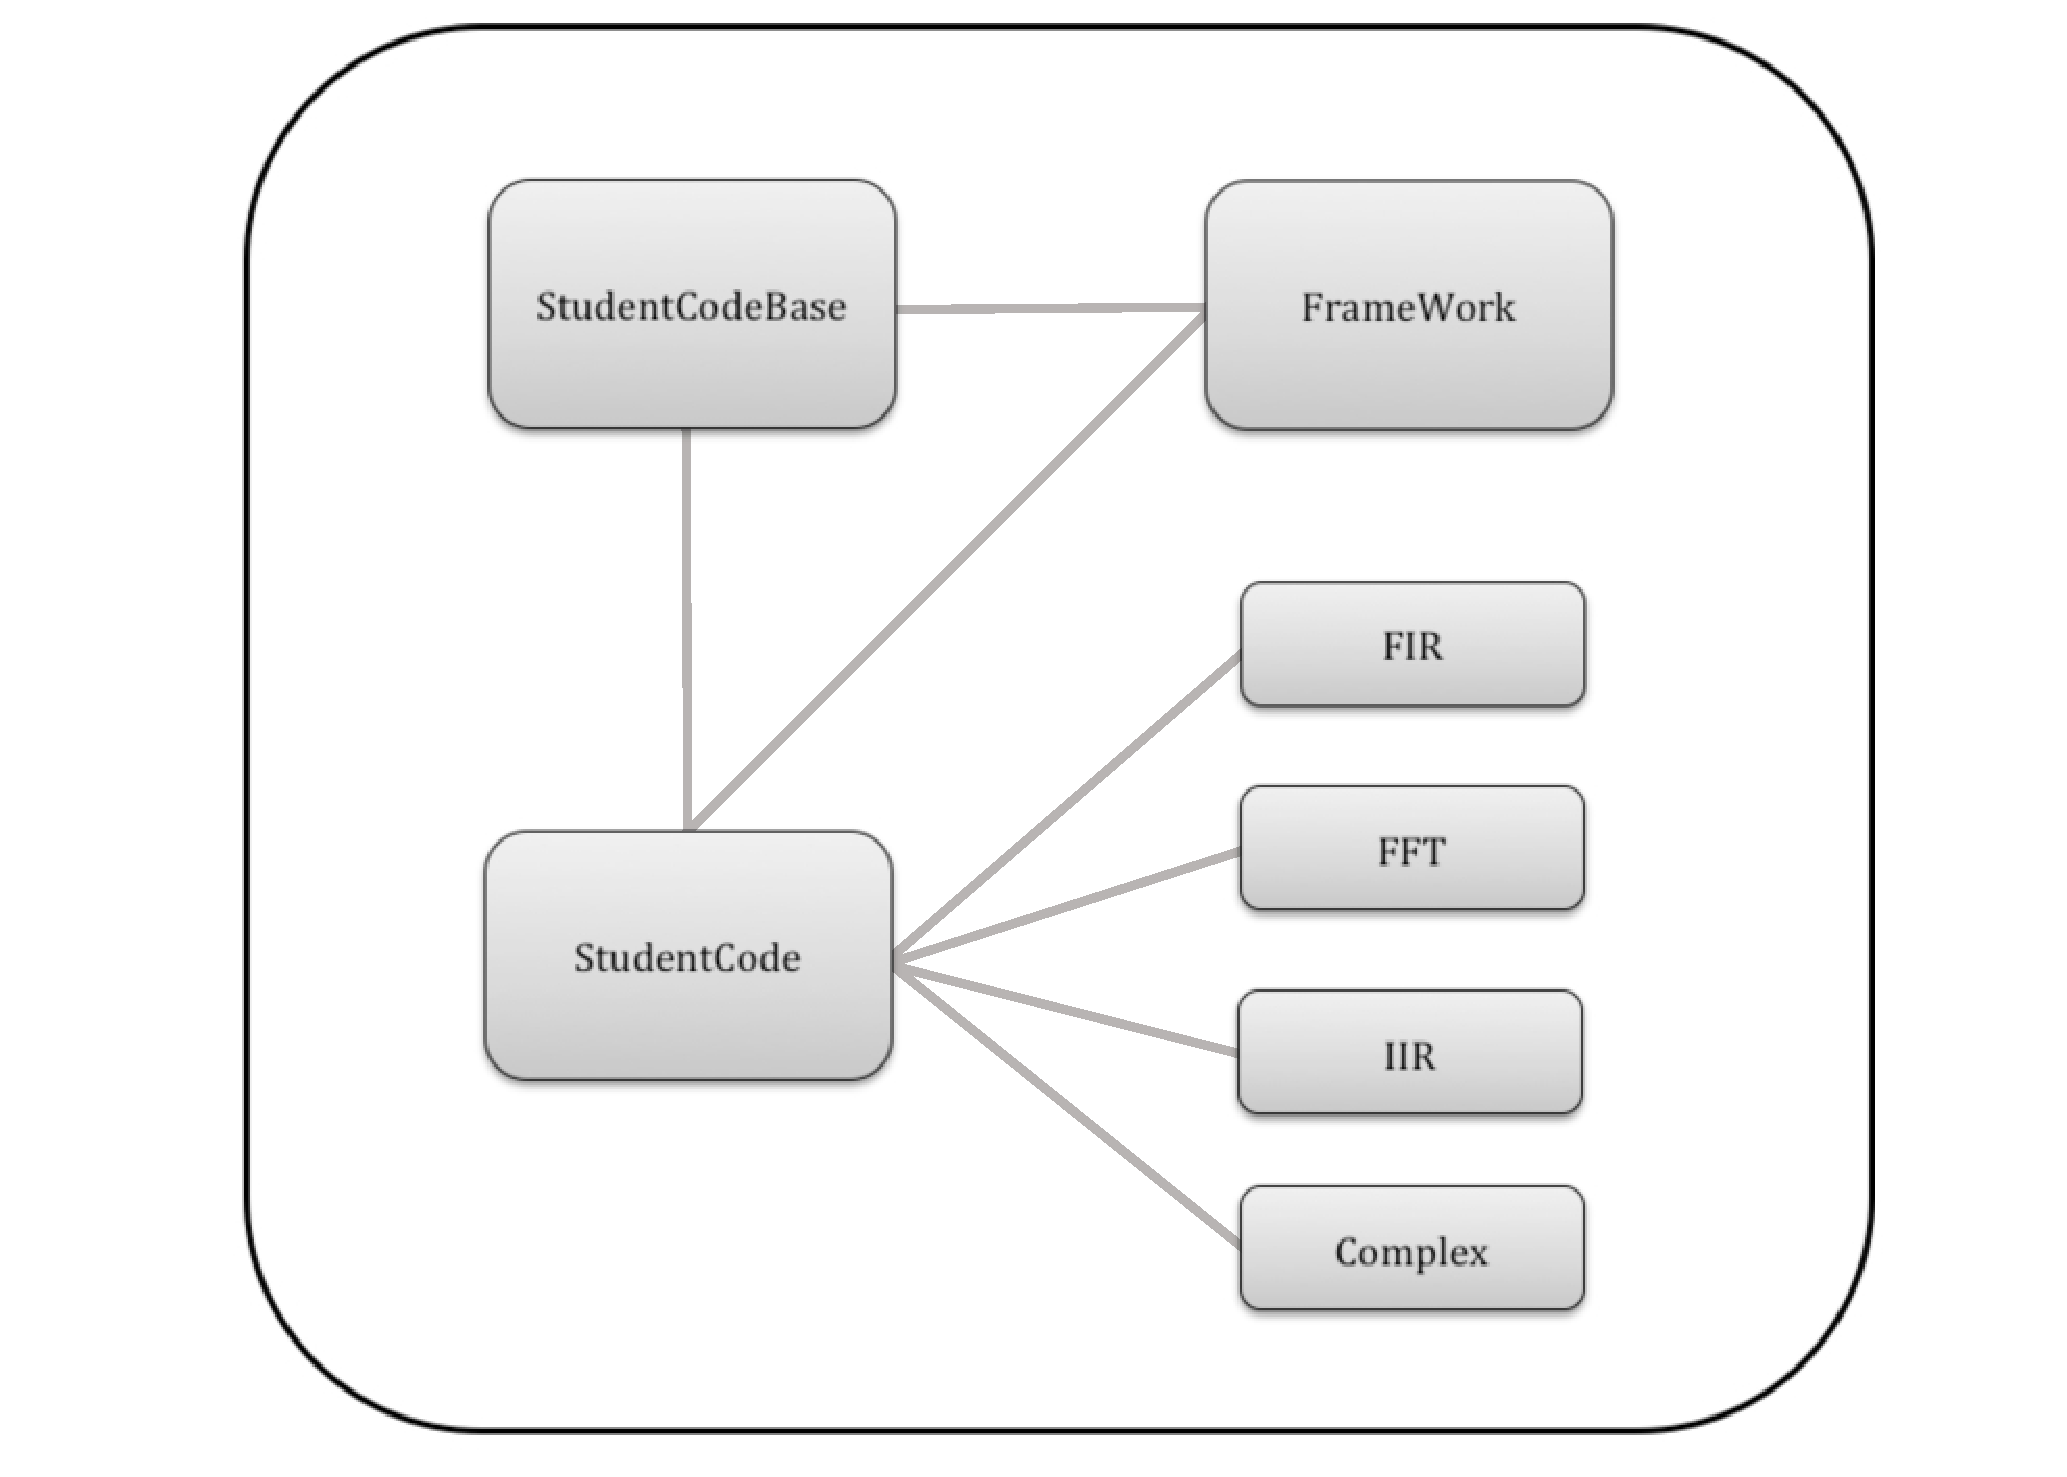
\includegraphics[width=0.9\textwidth]{FrameWorkPicture.pdf}
    \caption{Description of FrameWork. }
    \label{fig:FrameWorkPicture}
\end{figure}



\subsection{Transmitter and Receiver}

Since we are transmitting and receiving a file through a 3,5mm cable we used two phones, one to transmit the file and the other to receive it. When starting the application, right after the user is told to plug in the headset \textcolor{red}{[Figure X]}, \textcolor{red}{four alternatives are given (change if we change layout)}. The user can kill the app, go in to transmitter mode \textcolor{red}{[Figure XX]} or go in to receiver mode \textcolor{red}{[Figure XXX]}. The fourth option is to select a file, where the user selects the file to be transmitted \textcolor{red}{[Figure XXXX]}. 

\subsection{Schematics}

The system can be described by the schematics shown in Figure \ref{fig:SchematicsSystem}. The user first choose a file to be transmitted. After the wished file is selected, the phone pulls the file from the SD-Card and \textcolor{red}{[starts the coding/transcoding]}. The file which has been transmitted to a sequence of bits, is then modulated before it is passed through the channel. \textcolor{red}{When the transmission is done the transmitting phone is put in a waiting state} while the receiving phone is accepting the file and starts the demodulation of the received data. The last step before the storage of the file on the receiving SD-Card is the decoding where the received file is reconstructed. After the received phone has saved the file to the SD-Card \textcolor{red}{[the process is put in a waiting state]}.

 \begin{figure}[H]
  \centering
    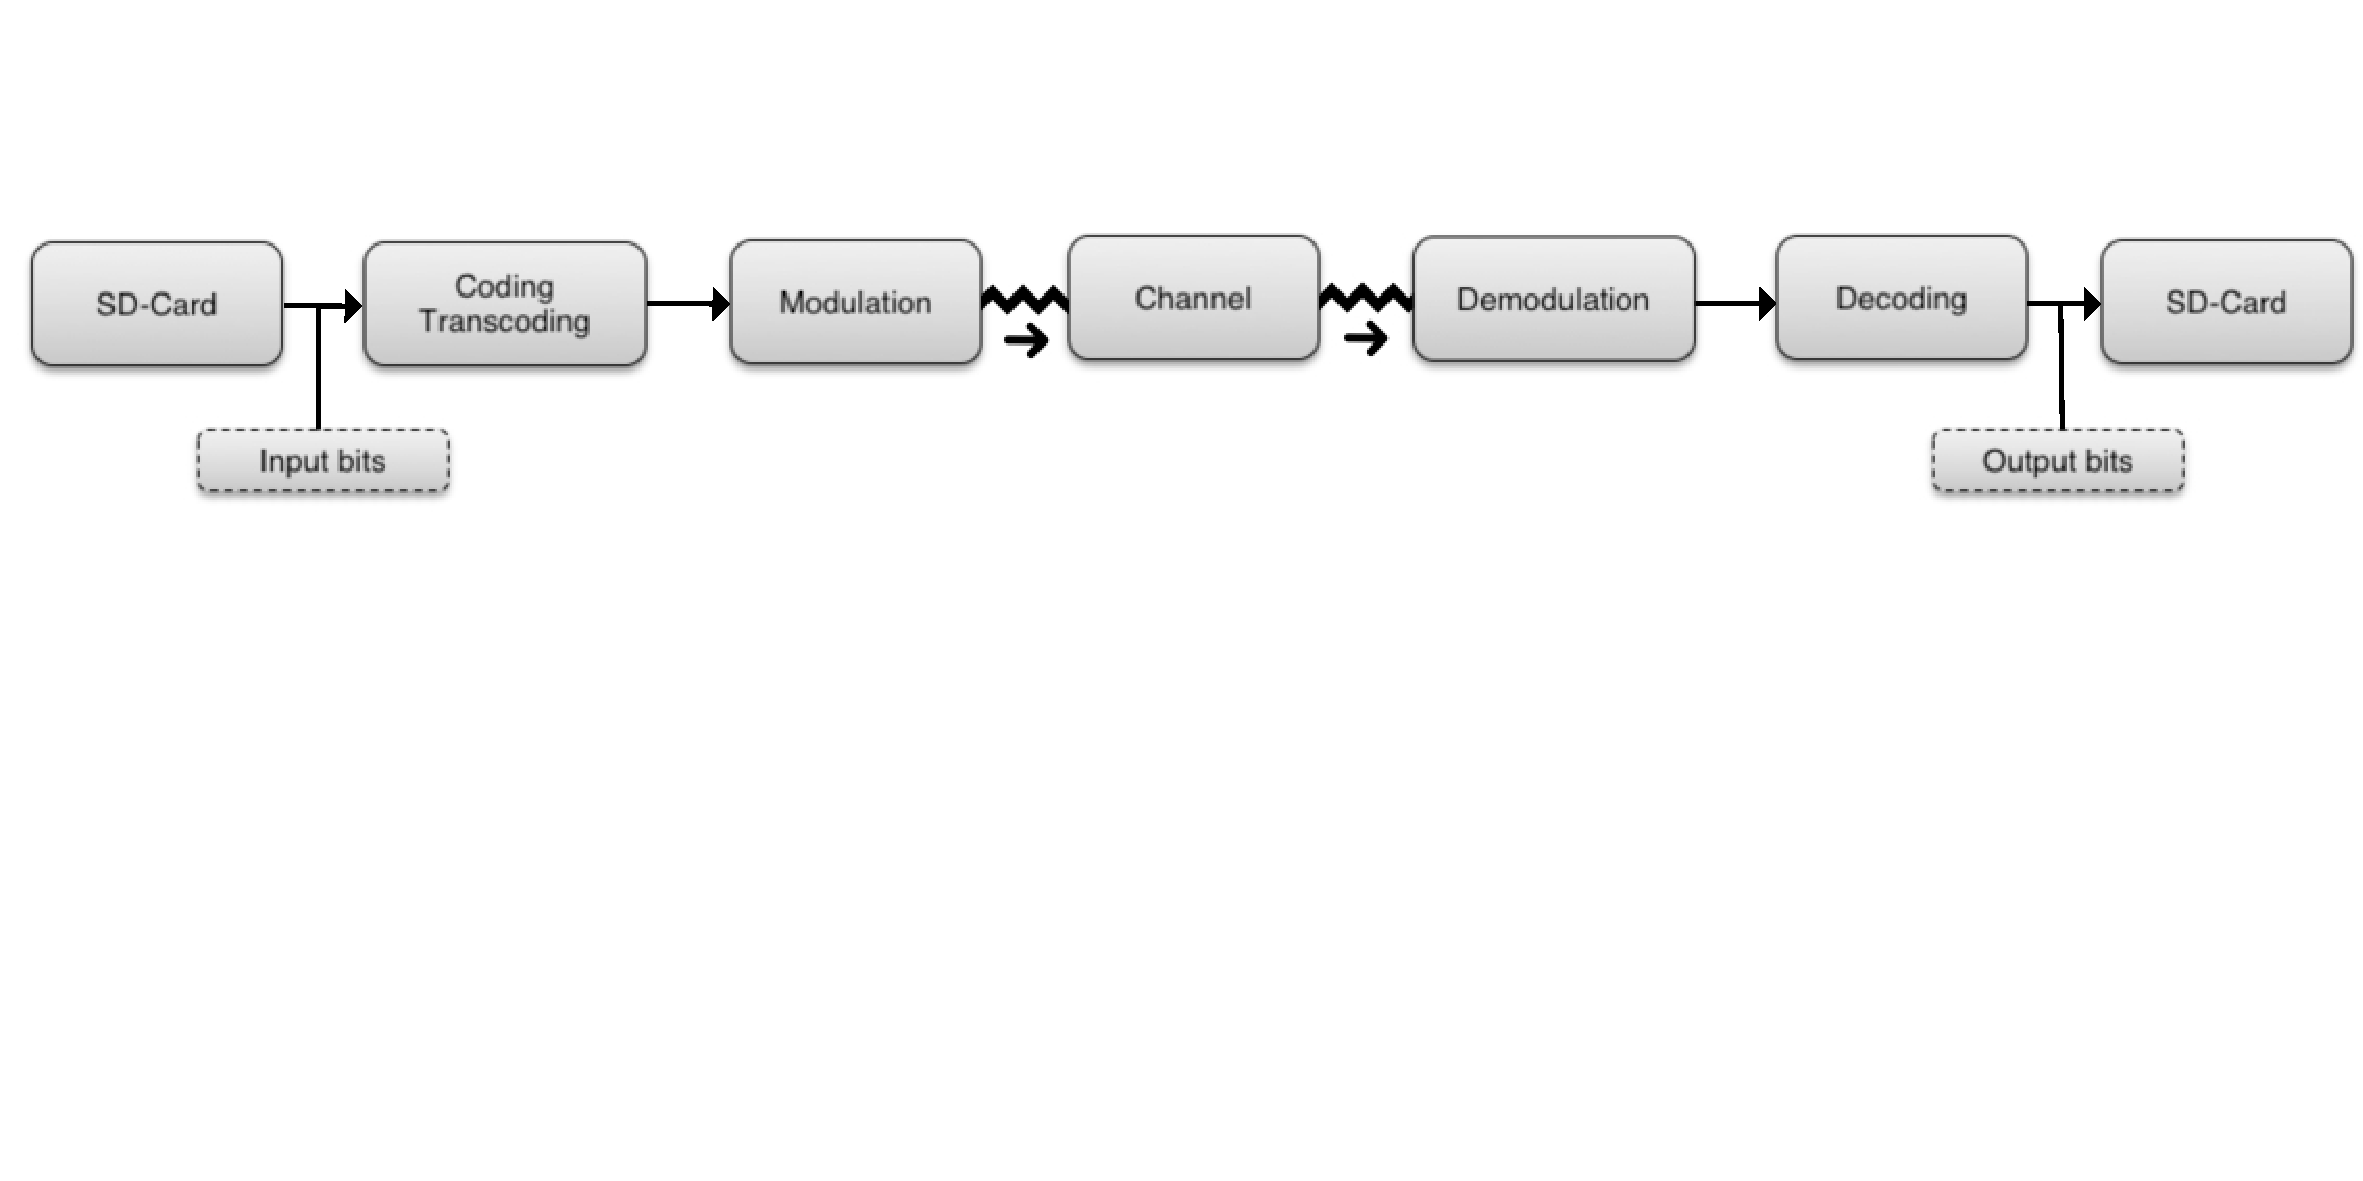
\includegraphics[width=0.9\textwidth]{SchematicsSystemForTheReport.pdf}
    \caption{Schematics system}
    \label{fig:SchematicsSystem}
\end{figure}

 
% % % % % % % % % % % % % % % % % % % % % % % % % % % % % % % % % % % % % % % % % % % % % % % % %
% % % % % % % % % % % % % % % % % % % % % % % % % % % % % % % % % % % % % % % % % % % % % % % %
\section{Performance Results}
We tested several modulations schemes modulating and demodulating random binary sequences, first with MATLAB (off-line mode), and then with the phones with the provided Android Framework (on-line mode). 
\subsection{Off-line testing}
Our first and basic test was to generate a random sequence and transmit it with binary FSK throughout the channel. As discussed in section \ref{sec:FSKdemod} , we used the Goertzel algorithm to decode the received modulated signal with generally good results.
 

\subsection{On-line testing}
%Include if possible BER results, processing time and some other observations in the real time implementation 
\clearpage


% % % % % % % % % % % % % % % % % % % % % % % % % % % % % % % % % % % 
% % % % % % % % % % % % % % % % % % % % % % % % % % % % % % % % % % %
\section{Conclusions}

\begin{thebibliography}{1}
\bibitem{Madhow}
Madhow U. \emph{Fundamentals of Digital Communication}, Cambridge , 2008.


\bibitem{Proakis}
Proakis J. ,Salehi Masoud, \emph{Digital Communications}, McGraw-Hill , 2008.
\bibitem{ASKDemGaza}
Abu M., \href{http://site.iugaza.edu.ps/mabufoul/files/2010/09/Experiment-5.pdf}
{\emph{ASK demodulator Lab Experiment}},
Islamic University of Gaza, retrieved in April 2014.


\bibitem{DigModTech}
Sa-nguankotchakorn T. , \href{http://www.tc.ait.ac.th/faculty/teerapat/AT77.11_Digital\%20Modulation\%20Techniques/III.Frequency_Shift_Keying.pdf}{\emph{Frequency Shift Keying Lecture Slides}}, Asian Institute of Technology, retrieved in April 2014.


\bibitem{DigCommLec}
Okechukwu C. Ugweje, \href{ugweje/web/Courses/Ee549/Handout/EE549F01Lecture37.pdf}{\emph{Frequency Shift Keying, Lecture Slides}},  University of Akron, retrieved in April 2014.



\bibitem{XiongDigModTech}
Xiong F., \emph{Digital Modulation Techniques}, Artech House, 2006.


\bibitem{gold}
Shembil S., \emph{M-Ary FSK with Orthogonal Pulse Envelopes and its Noncoherent Detection}, IJECS-IJENS, Vol. 10, No.06, Issued December 2010, pp. 103-106.

\bibitem{GoertzelPaper}
Sysel and Rajmic, \emph{Goertzel algorithm generalized to non-integer multiples of fundamental frequency}, EURASIP Journal on Advances in Signal Processing, 2012, 2012:56.
\bibitem{ProjectEQ2310}
Project Assignment EQ2310 Digital Communications, \emph{Analysis and Simulation of a QPSK System}, KTH, 2013.

\bibitem{HaykinBook}
Haykin S., \emph{Digital Communication Systems}, John Wiley \& Sons, Inc., 2014.

\bibitem{CarrierSynchPaper}
Dick D., Harris F., and Rice M., \emph{FPGA Implementation of Carrier Synchronization for QAM Receivers}, Journal of VLSI Signal Processing 36, 57-71, 2004.

\bibitem{FFTJavaRef} 
Sedgewick R., and Wayne K.,
\href{http://introcs.cs.princeton.edu/java/97data/FFT.java.html}{\emph{FFT.java}},  Princeton
Copyright © 2000–2011

\bibitem{ComplexJavaRef} 
Sedgewick R., and Wayne K.,
\href{http://introcs.cs.princeton.edu/java/97data/Complex.java.html}{\emph{Complex.java}},  Princeton
Copyright © 2000–2011


\bibitem{SklarBook}
Sklar B. \emph{Digital Communications Fundamentals and Applications}, Prentice Hall, 2001.


%% Slides & handouts



\end{thebibliography}


\end{document}
